\chapter{Graph-Datenbanken im praktischen Einsatz: OLAP}
\section{PostgreSQL: OLAP}
Im folgenden Abschnitt werden die in Kapitel 3 vorgestellten SQLs auf ihre Leistungsfähigkeit untersucht. Für die Messung wurden vier verschiedene Stored Procedures angelegt:
\begin{itemize}
	\item innerJoinGenerator
	\item recursivesearch
	\item selectCascadingGenerator
	\item selectUnionGenerator
\end{itemize}
Der Aufruf der Statements funktioniert gleich, es werden die Rekursionstiefe, der Startknoten und die Tabelle, auf welcher die Stored Procedure ausgeführt wird, übergeben.

Die Funktionen innerJoinGenerator, selectCascadingGenerator und selectWithUnionSourceCodeGenerator generieren die entsprechenden Statements und führen diese aus. Die Funktion innerJoinGenerator erzeugt ein Select Statement in der die Abfrage, wie in Abschnitt \ref{postgresInnerJoin} beschrieben, erzeugt und ausgeführt wird. Entsprechend erzeugt selectCascadingGenerator eine verschachtelte Select-Abfrage. Die Funktion ist in Listing \ref{StandardSQLGenerisch} abgebildet. Die Funktion selectUnionGenerator erzeugt eine Abfrage wie in Abschnitt \ref{postgresStandardSQL} beschrieben. Bei der Funktion recursivesearch handelt es sich um die Funktion wie sie in Abschnitt \ref{postgresRecursiveFunction} beschrieben.

\subsection{Indexe und Partionierte Tabellen}
Um eine bessere Aussage über die Performance von PostgreSQL zu bekommen wurden zusätzlich zu den ''Default'' --Relationstabellen für jeden Datensatz zwei weitere Tabellen angelegt.

Die erste Tabelle hat das Suffix ''\_with\_index''. Im Listing ist Beispielhaft das Create-Skript für die Relationen aus dem Datensatz ''youtube'' dargestellt:

\lstsetsql
\begin{lstlisting}[language=SQL,caption = Tabelle mit Index anlegen,frame=single, label={lineInQueryPlan} ]
CREATE TABLE IF NOT EXISTS relation_youtube_with_index(
src INTEGER REFERENCES profiles_youtube(ID),
dst INTEGER REFERENCES profiles_youtube(ID),
type VARCHAR(50),
date DATE
);
CREATE INDEX yt_dst ON relation_youtube_with_index (dst);
CREATE INDEX yt_src ON relation_youtube_with_index (src);
\end{lstlisting}

Im Unterschied zur ''public\_youtube''--Tabelle wurde diese Tabelle noch um Zwei Indices erweitert. Dabei wurde ein index auf die src-Spalte angelegt, der andere auf die dst-Spalte.


Neben der den ''\_with\_index''--Tabellen wurden noch die \_partitioned--Tabellen angelegt. Diese verwenden die gleichen Indices wie die ''\_with\_index''-Tabellen, jedoch sind sie zusätzlich in 4 Partitonen aufgteilt:

\begin{lstlisting}[language=SQL,caption = Partitonierte Tabelle mit Indices anlegen,frame=single, label={lineInQueryPlan} ]

CREATE TABLE IF NOT EXISTS relation_youtube_partitioned(
src INTEGER REFERENCES profiles_youtube(ID),
dst INTEGER REFERENCES profiles_youtube(ID),
type VARCHAR(50),
date DATE
)PARTITION BY RANGE(src);
CREATE INDEX yt_part_src ON relation_youtube_partitioned (src);
CREATE INDEX yt_part_dst ON relation_youtube_partitioned (dst);
CREATE TABLE relation_youtube_partitioned_0 PARTITION OF relation_youtube_partitioned
FOR VALUES FROM (0) TO (800000);
CREATE TABLE relation_youtube_partitioned_1 PARTITION OF relation_youtube_partitioned
FOR VALUES FROM (800001) TO (1600000);
CREATE TABLE relation_youtube_partitioned_2 PARTITION OF relation_youtube_partitioned
FOR VALUES FROM (1600001) TO (2400000);
CREATE TABLE relation_youtube_partitioned_3 PARTITION OF relation_youtube_partitioned
FOR VALUES FROM (2400001) TO (3200000);
\end{lstlisting}

Da die Datensätze unterschiedlich groß sind wurden die Partionsgrößen entsprechend angepasst. Jeder Datensatz wurde auf 4 Partitonen verteilt. Damit ergibt sich für den Datensatz youtube eine Partitonsgröße von 800.000.



\subsection{Benchmark}
Mit der Standardinstallation von PostgreSQL wird auch pgbench mitinstalliert. Bei pgbench handelt es sich um ein einfaches Tool zur Durchführung von Benchmark-Tests. Bei einem Benchmark-Test wird eine Menge von \ac{SQL}-Statements beliebig oft wiederholt, dabei können auch mehrere parallele Sessions geöffnet werden. Beim durchführen des Tests berechnet pgbench die durchschnittliche Latenz aller Requests, sowie die Transaktionen pro Sekunde.
\subsubsection{Verwendung von pgbench}
pgbench wird über die Kommandozeile gestartet. Dabei können eine Reihe von Parametern übergeben werden, mit denen das Verhalten von pgbench gesteuert werden kann.
\begin{itemize}
	\item -c clients  \\
	Über das Flag -c wird die Anzahl der Clients bzw. die Anzahl der gleichzeitigen Datenbankverbindungen festgelegt. Wenn hier nichts angegeben ist wird nur ein Client verewendet.
	\item -t transactions \\
	Über das Flag -t wird festgelegt wieviele Transaktionen jeder Client durchführt. Die Anzahl aller Transaktionen ergibt sich durch das Produkt von Clients und Transactions.
	\item -h hostname \\
	Der Hostname des Datenbankservers.
	\item -p Port \\
	Der Port auf dem die Datenbank hört.
	\item -U login \\
	Der Nutzername mit dem sich pgbench anmeldet. Hier kann kein Passwort angegeben werden. Das Datenbankpasswort kann in die Systemvariable PGPASSWORD geschrieben werden. Diese Varibale wird von pgbench dann ausgwewertet.
	\item -d Database \\
	Die Datenbank gegen die sich pgbench verbindet
	\item -f File \\ 
	Über -f kann jeweils eine Datei mit mehreren SQL-Statements übergeben werden. Eine Transaktion entspricht dabei der Abarbeitung aller SQL-Befehle innerhalb der Datei.
	Wird keine Datei angegeben führt pgbench ein Default-Benchmarking aus.

\end{itemize}
Für die Benchmarktests wurden zehn Clients parallel gestartet werden, die jeweils fünf Transaktionen durchführen sollten. Aus dem Mittelwert dieser 50 Transaktionen wurden bestimmt pgbench Latenz und Transaktionen pro Sekunde.

\begin{lstlisting}[language=bash,caption = pgbench Statment,frame=single, label={lineInQueryPlan} ]
/usr/lib/postgresql/11/bin/pgbench \ 
-h 10.20.110.43 -p 5413 \ 
-U postgres -d team22 \ 
-c 10 -t 5 -f Select_innerjoinsourcecodegenerator_1.sql
\end{lstlisting}
Pgbench kann kein Passwort übergeben werden. Als Workaround kann das Passwort in die Umgebungsvariable PGPASSWORD gespeichert werden. Die Variable wird dann von pgbench ausgewertet. 
\subsubsection{Testaufbau}
Für die Benchmarktests wurde auf dem Master-Node der Ordner pgbench angelegt. Im Ordner pgbench sind eine Reihe von Unterordnern angelegt sowie das Skript pgbench.sh. Dieses Skript erzeugt das pgbench-Statment. Anschließend ruft das Skript sequentiell alle pgbensh.sh-Skripte auf die sich in den Unterordnern befinden auf.
\begin{figure}[H]
\tikzstyle{every node}=[draw=black,thick,anchor=west]
\usetikzlibrary{trees}
\tikzstyle{file}=[draw=none]
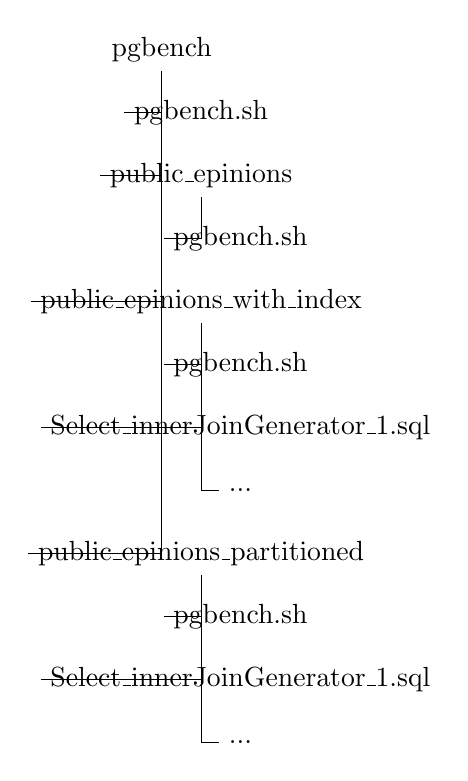
\begin{tikzpicture}[%
grow via three points={one child at (0.5,-0.8) and
	two children at (0.5,-0.8) and (0.5,-1.6)},
edge from parent path={(\tikzparentnode.south) |- (\tikzchildnode.west)}]
\node {pgbench}
child{ node[file]{pgbench.sh}}
child { node {public\_epinions}
	child{ node[file]{pgbench.sh}}
}
child [missing] {}		
child { node {public\_epinions\_with\_index}
child{ node[file]{pgbench.sh}}
child{node[file]{Select\_innerJoinGenerator\_1.sql}}
child{node[file]{...}}
}
child [missing] {}
child [missing] {}
child [missing] {}	
child { node {public\_epinions\_partitioned}
child{ node[file]{pgbench.sh}}
child{node[file]{Select\_innerJoinGenerator\_1.sql}}
child{node[file]{...}}
};
\end{tikzpicture}
%Reset Configuration
\tikzstyle{every node}=[]
\caption{Ordnerstruktur Benchmarktest}
\end{figure}
Jedes pgbench.sh-Skript startet sequenziell einen pgbench-Benchmarktest mit jeder SQL-Datei im selben Ordner. Jeder Ordner steht dabei für eine der relations-Tabellen. Für jede Kombination aus Rekursionstiefe und SQL-Statement gibt es eine SQL-Datei, welche genau ein Statement enthält.

Nach jedem Durchlauf von pgbench wird folgende Ausgabe erzeugt:

\begin{lstlisting}[caption= Ausgabe pgbench]
pghost: 10.20.110.43 pgport: 5413 nclients: 10 nxacts: 5 dbName: team22
transaction type: Select_innerjoinsourcecodegenerator_1.sql
scaling factor: 1
query mode: simple
number of clients: 10
number of threads: 1
number of transactions per client: 5
number of transactions actually processed: 50/50
latency average = 9.899 ms
tps = 1010.157069 (including connections establishing)
tps = 1104.908743 (excluding connections establishing)
\end{lstlisting}

Der Output von pgbench wird mit Hilfe der pgbench.sh Skripte in eine Logdatei geschrieben. Die Logdatei wird innerhalb jedes Ordners unterhalb von pgbench angelegt.
Für jeden Testlauf wird eine neue Logdatei angelegt. Damit die Logdateien nicht überschrieben werden, wird die Logdatei mit einem Zeitstempel angelegt. So steht zum Beispiel in der Datei unter dem Pfad
 \texttt{/pgbench/public\_epinions\_with\_index /pgbench\_2019\_01\_12\_15\_26.log} die Ausgabe des Benchmarktests für die Tabelle \texttt{public\_epionions\_with\_index} vom 12.1.2019.
 
 In den folgenden drei Abschnitten sind die durchschnittlichen Latenzen aller Tabellen dargestellt. Die Unterteilung erfolgt hierbei nach Tabellen ohne Indices, Tabellen mit Incides und  Partionierte Tabellen mit Indices. 

\newpage
\subsubsection{Antwortzeiten ohne Indices}
In diesem Abschnitt sind die Laufzeiten der verschiedenen SQLs auf den Tabellen ohne Indices dargestellt.
\paragraph{relation\_epinions}\mbox{}\\
\begin{figure}[H]
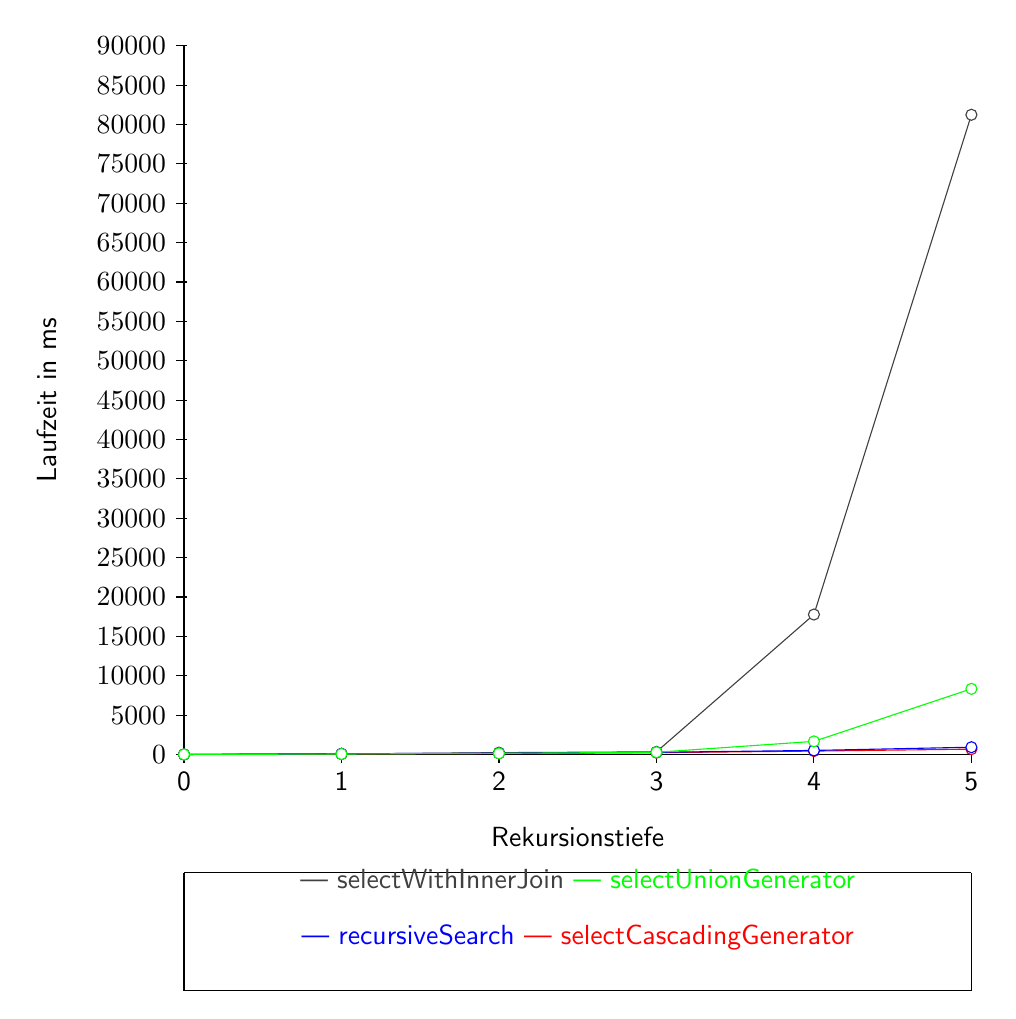
\begin{tikzpicture}[y=.5cm, x=2cm,font=\sffamily]
%axis
\draw (0,0) -- coordinate (x axis mid) (5,0);
\draw (0,0) -- coordinate (y axis mid) (0,18);
    	%ticks
\foreach \x in {0,...,5}
\draw (\x,1pt) -- (\x,-3pt)
node[anchor=north] {\x};
	\foreach \y/\ytext in {
	0/0,
	1/5000,
	2/10000,
	3/15000,
	4/20000,
	5/25000,
	6/30000,
	7/35000,
	8/40000,
	9/45000,
	10/50000,
	11/55000,
	12/60000,
	13/65000,
	14/70000,
	15/75000,
	16/80000,
	17/85000,
	18/90000
}
\draw (1pt,\y) -- (-3pt,\y) node[anchor=east] {$\ytext$}; 
%labels      
\node[below=0.8cm] at (x axis mid) {Rekursionstiefe};
\node[rotate=90, above=1.5cm] at (y axis mid) {Laufzeit in ms};
%plots
\draw[darkgray] plot[ mark=*, mark options={fill=white}] 
coordinates{(0, 0)
	(1, 61.065/5000)
	(2,231.850/5000)
	(3,333.011/5000)
	(4,3.5545)%17772.456/5000)
	(5,16.2483)%81241.284/5000
};

\draw[red] plot[ mark=*, mark options={fill=white}] 
coordinates{(0, 0)
			(1, 63.636/5000)
			(2,139.225/5000)
			(3,229.997/5000)
			(4,432.297/5000)
			(5,677.420/5000)
		};
\draw[blue] plot[ mark=*, mark options={fill=white}] 
coordinates{(0, 0)
	(1, 89.858/5000)
	(2,168.822/5000)
	(3,273.452/5000)
	(4,513.038/5000)
	(5,921.228/5000)
};
\draw[green] plot[ mark=*, mark options={fill=white}] 
coordinates{(0, 0)
	(1, 59.275/5000)
	(2,143.367/5000)
	(3,277.766/5000)
	(4,1664.168/5000)
	(5,8335.513/5000)
};
\draw (0,-3) -- (5,-3) 
(0,-3) -- (0,-6)
(0,-6) -- (5,-6)
(5,-3) -- (5,-6);
\draw[draw=none] (0,0) -- (5,0) 
node[draw=none, midway, yshift=-4.5em]
{
	\textcolor{darkgray}{--- selectWithInnerJoin}
	\textcolor{green}{--- selectUnionGenerator} 
	
};
\draw[draw=none] (0,-3) -- (5,0) 
node[draw=none, midway, yshift=-4.5em]
{
	\textcolor{blue}{--- recursiveSearch} 
	\textcolor{red}{--- selectCascadingGenerator}
};
\end{tikzpicture}
	\caption{ relation\_epinions}
\end{figure}

% Please add the following required packages to your document preamble:
% \usepackage{multirow}
\begin{table}[H]
	\begin{tabular}{l|l|l|l|l|l|}
		\cline{2-6}
		& \multicolumn{5}{|l|}{Laufzeit in MS}                                                                                                                                                  \\ \hline
		\multicolumn{1}{|l|}{\multirow{2}{2cm}{Rerkusions-tiefe}} & \multicolumn{2}{|l|}{\multirow{2}{3cm}{selectCascading Generator}} & \multirow{2}{2.8cm}{recursiveSearch} & \multirow{2}{2.5cm}{selectUnion Generator} & \multirow{2}{2.5cm}{selectInner JoinGenerator} \\
		\multicolumn{1}{|l|}{}
		& \multicolumn{2}{|l|}{}                                           &                                  &                                     &                                           \\ \hline
	\multicolumn{1}{|l|}{1}               & \multicolumn{2}{l|}{63.636}                                     & 89.858                           & 59.275                              & 61.065                                    \\ \hline
	\multicolumn{1}{|l|}{2}               & \multicolumn{2}{l|}{139.225}                                    & 168.822                          & 143.367                             & 231.850                                   \\ \hline
	\multicolumn{1}{|l|}{3}               & \multicolumn{2}{l|}{229.997}                                    & 273.452                          & 277.766                             & 333.011                                   \\ \hline
	\multicolumn{1}{|l|}{4}               & \multicolumn{2}{l|}{432.297}                                    & 513.038                          & 1664.168                            & 17772.456                                 \\ \hline
	\multicolumn{1}{|l|}{5}               & \multicolumn{2}{l|}{677.420}                                    & 921.228                          & 8335.513                            & 81241.284                                 \\ \hline
	
	\end{tabular}
	\caption{Laufzeit der SQLs für Tabelle relation\_epions}
\end{table}

Bei der relation\_epinions Tabelle zeigen sich ab der 3. Rekursionstufe deutliche Unterschiede in den Laufzeiten der einzelnen Statements. In der Rekursionsstufe 5 schneidet das Innerjoin-Statement mit 81 Sekunden am schlechtesten ab. Das verschachtelte Select ist mit 677 Millisekunden am schnellsten und benötigt dabei nur 
0.8\% der Laufzeit des Innerjoin Statements.

\paragraph{relation\_livejournal}\mbox{}\\

\begin{figure}[H]

	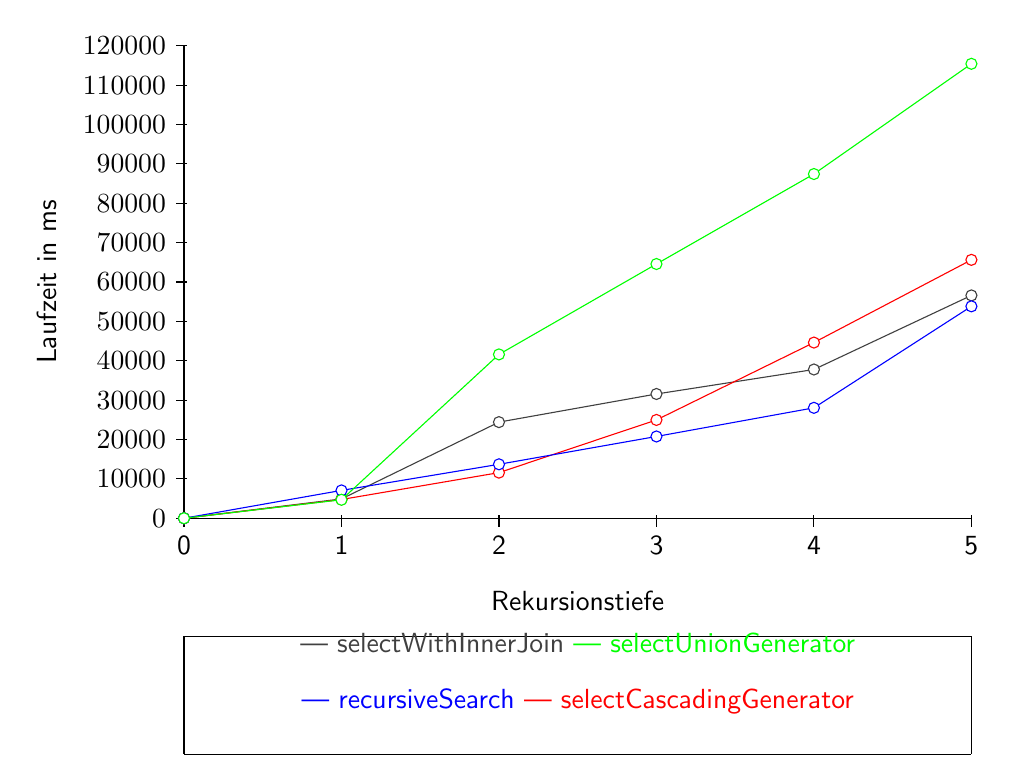
\begin{tikzpicture}[y=.25cm, x=2cm,font=\sffamily]
	%axis
	\draw (0,0) -- coordinate (x axis mid) (5,0);
	\draw (0,0) -- coordinate (y axis mid) (0,24);
	%ticks
	\foreach \x in {0,...,5}
	\draw (\x,1pt) -- (\x,-3pt)
	node[anchor=north] {\x};
	\foreach \y/\ytext in {
		0/0,	
		2/10000,
		4/20000,
		6/30000,
		8/40000,
		10/50000,
		12/60000,
		14/70000,
		16/80000,
		18/90000,
		20/100000,
		22/110000,
		24/120000
	}
	\draw (1pt,\y) -- (-3pt,\y) node[anchor=east] {$\ytext$};
	%labels      
	\node[below=0.8cm] at (x axis mid) {Rekursionstiefe};
	\node[rotate=90, above=1.5cm] at (y axis mid) {Laufzeit in ms};
	%plots
	\draw[darkgray] plot[mark=*, mark options={fill=white}] 
	coordinates{(0, 0)
		(1, 0.9819)%4909.862/5000)
		(2,	4.8836)%24417.787/5000)
		(3, 6.3127)%31563.339/5000)
		(4, 7.5570)%37785.200/5000)
		(5,	11.3202)%56601.185/5000)
	};
	\draw[red] plot[mark=*, mark options={fill=white}] 
	coordinates{(0, 0)
		(1, 4761.733/5000)
		(2,	11589.219/5000)
		(3, 4.9944)	%=24971/5000
		(4, 8.9252) %=44625,935÷5000
		(5,	13.1265944)%=65632,972÷5000
	};
\draw[blue] plot[mark=*, mark options={fill=white}] 
coordinates{(0, 0)
	(1, 1.4151)%7075.399/5000)
	(2,	2.7405)%13702.381/5000)
	(3, 4.1548)%20773.827/5000)
	(4, 5.6098)%28048.866/5000)
	(5,	10.7651)%53825.401/5000)
};
\draw[green] plot[mark=*, mark options={fill=white}] 
coordinates{(0, 0)
	(1, 0.939)%4695.466/5000)
	(2,	8.323)%41616.216/5000)
	(3, 12.916)%64577.873/5000)
	(4, 17.487)%87434.075/5000)	
	(5,	23.086)%115432.071/5000)	
};
	\draw (0,-6) -- (5,-6) 
(0,-6) -- (0,-12)
(0,-12) -- (5,-12)
(5,-6) -- (5,-12);
\draw[draw=none] (0,0) -- (5,0) 
node[draw=none, midway, yshift=-4.5em]
{
	\textcolor{darkgray}{--- selectWithInnerJoin}
	\textcolor{green}{--- selectUnionGenerator} 
	
};
\draw[draw=none] (0,-6) -- (5,0) 
node[draw=none, midway, yshift=-4.5em]
{
	\textcolor{blue}{--- recursiveSearch} 
	\textcolor{red}{--- selectCascadingGenerator}
};
	\end{tikzpicture}
	\caption{ relation\_livejournal}
\end{figure}
\begin{table}[H]
	\begin{tabular}{l|l|l|l|l|l|}
		\cline{2-6}
		& \multicolumn{5}{|l|}{Laufzeit in MS}                                                                                                                                                  \\ \hline
		\multicolumn{1}{|l|}{\multirow{2}{2cm}{Rerkusions-tiefe}} & \multicolumn{2}{|l|}{\multirow{2}{3cm}{selectCascading Generator}} & \multirow{2}{2.8cm}{recursiveSearch} & \multirow{2}{2.5cm}{selectUnion Generator} & \multirow{2}{2.5cm}{selectInner JoinGenerator} \\
		\multicolumn{1}{|l|}{}
		& \multicolumn{2}{|l|}{}                                           &                                  &                                     &                                           \\ \hline
		\multicolumn{1}{|l|}{1}                                 & \multicolumn{2}{l|}{4761.733}                                    & 7075.399                                              & 4695.466                                                  & 4909.862                                                        \\ \hline
		\multicolumn{1}{|l|}{2}                                 & \multicolumn{2}{l|}{11589.219}                                   & 13702.381                                             & 41616.216                                                 & 24417.787                                                       \\ \hline
		\multicolumn{1}{|l|}{3}                                 & \multicolumn{2}{l|}{24971}                                       & 20773.831                                             & 64577.873                                                 & 31563.339                                                       \\ \hline
		\multicolumn{1}{|l|}{4}                                 & \multicolumn{2}{l|}{44625.935}                                   & 28048.866                                             & 87434.075                                                 & 37785.200                                                       \\ \hline
		\multicolumn{1}{|l|}{5}                                 & \multicolumn{2}{l|}{65632.972}                                   & 53825.401                                             & 115432.071                                                & 56601.185                                                       \\ \hline
		
	\end{tabular}
	\caption{Laufzeit der SQLs für Tabelle relation\_livejournal}
\end{table}

Bei der relation\_livejournal Tabelle sind die Laufzeiten am längsten. Hier schneidet das Standard-SQL am schlechtesten ab. Die Rekursive Stored Procedure ist hier am schnellsten. Jedoch sind die Laufzeiten in der fünften Rekursionsstufe mit im besten Fall 53 Sekunden und im schlechtesten Fall 115 Sekunden sehr lange. Selbst in der ersten Rekursionstufe benötigt eine Abfrage mindestens 4,6 Sekunden.

\paragraph{relation\_facebook}\mbox{}\\

\begin{figure}[H]
	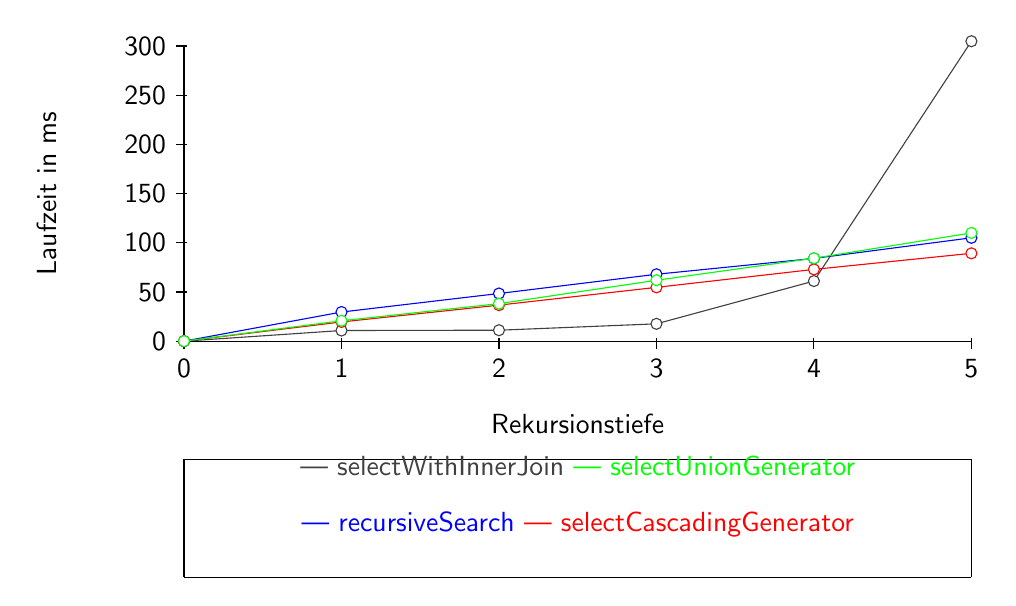
\begin{tikzpicture}[y=.0125cm, x=2cm,font=\sffamily]
	%axis
	\draw (0,0) -- coordinate (x axis mid) (5,0);
	\draw (0,0) -- coordinate (y axis mid) (0,300);
	%ticks
	\foreach \x in {0,...,5}
	\draw (\x,1pt) -- (\x,-3pt)
	node[anchor=north] {\x};
	\foreach \y in {0,50,...,300}
	\draw (1pt,\y) -- (-3pt,\y)
	node[anchor=east] {\y}; 
	%labels      
	\node[below=0.8cm] at (x axis mid) {Rekursionstiefe};
	\node[rotate=90, above=1.5cm] at (y axis mid) {Laufzeit in ms};
	%plots
	\draw[darkgray] plot[ mark=*, mark options={fill=white}] 
	coordinates{(0, 0)
		(1, 10.825)
		(2, 11.119)
		(3, 17.613)
		(4, 61.089)
		(5, 304.821)
	};
	
	\draw[blue] plot[ mark=*, mark options={fill=white}] 
	coordinates{(0, 0)
		(1, 29.595)
		(2,48.442)
		(3,67.989)
		(4,84.084)
		(5,105.049)
	};
	\draw[red] plot[ mark=*, mark options={fill=white}] 
	coordinates{(0, 0)
		(1, 19.528)
		(2,36.613)
		(3,54.681)
		(4,72.934)
		(5,89.262)
	};
	\draw[green] plot[ mark=*, mark options={fill=white}] 
	coordinates{(0, 0)
		(1, 20.716)
		(2,38.137)
		(3,61.904)
		(4,84.295)
		(5,110.000)
	};

	\draw (0,-120) -- (5,-120) 
		  (0,-120) -- (0,-240)
          (0,-240) -- (5,-240)
          (5,-120) -- (5,-240);
\draw[draw=none] (0,0) -- (5,0) 
node[draw=none, midway, yshift=-4.5em]
{
	\textcolor{darkgray}{--- selectWithInnerJoin}
	\textcolor{green}{--- selectUnionGenerator} 
	
};
\draw[draw=none] (0,-120) -- (5,0) 
node[draw=none, midway, yshift=-4.5em]
{
	\textcolor{blue}{--- recursiveSearch} 
	\textcolor{red}{--- selectCascadingGenerator}
};
	\end{tikzpicture}
	\caption{ relation\_facebook}
\end{figure}

\begin{table}[H]
	\begin{tabular}{l|l|l|l|l|l|}
		\cline{2-6}
		& \multicolumn{5}{|l|}{Laufzeit in MS}                                                                                                                                                  \\ \hline
		\multicolumn{1}{|l|}{\multirow{2}{2cm}{Rerkusions-tiefe}} & \multicolumn{2}{|l|}{\multirow{2}{3cm}{selectCascading Generator}} & \multirow{2}{2.8cm}{recursiveSearch} & \multirow{2}{2.5cm}{selectUnion Generator} & \multirow{2}{2.5cm}{selectInner JoinGenerator} \\
		\multicolumn{1}{|l|}{}
		& \multicolumn{2}{|l|}{}                                           &                                  &                                     &                                           \\ \hline
		\multicolumn{1}{|l|}{1}                                 & \multicolumn{2}{l|}{19.528}                                      & 29.595                                                & 20.716                                                    & 10.825                                                          \\ \hline
		\multicolumn{1}{|l|}{2}                                 & \multicolumn{2}{l|}{36.613}                                      & 48.442                                                & 38.137                                                    & 11.119                                                          \\ \hline
		\multicolumn{1}{|l|}{3}                                 & \multicolumn{2}{l|}{54.681}                                      & 67.989                                                & 61.904                                                    & 17.613                                                          \\ \hline
		\multicolumn{1}{|l|}{4}                                 & \multicolumn{2}{l|}{72.934}                                      & 84.084                                                & 84.295                                                    & 61.089                                                          \\ \hline
		\multicolumn{1}{|l|}{5}                                 & \multicolumn{2}{l|}{89.262}                                      & 105.049                                               & 110.000                                                   & 304.821                                                         \\ \hline
		
		
	\end{tabular}
	\caption{Laufzeit der SQLs für Tabelle relation\_facebook}
\end{table}

Bei den facebook-Daten ist das Laufzeitverhalten des verschachtelten Selects, der rekursiven Funktion und dem Standard SQL gleich. Die Unterschiede in der Latenz sind im Verhältnis zur Latenz gering. Einen Sonderfall bildet das innerJoin hier ist ab der dritten Rekursionsstufe ein exponentieller Anstieg der Laufzeit zu beobachten. Ab der ersten bis zur einschlieĺich vierten Rekursionstufe ist das innerJoin jedoch am Performantesten.

\newpage

\paragraph{relation\_wiki\_vote}\mbox{}\\

\begin{figure}[H]
	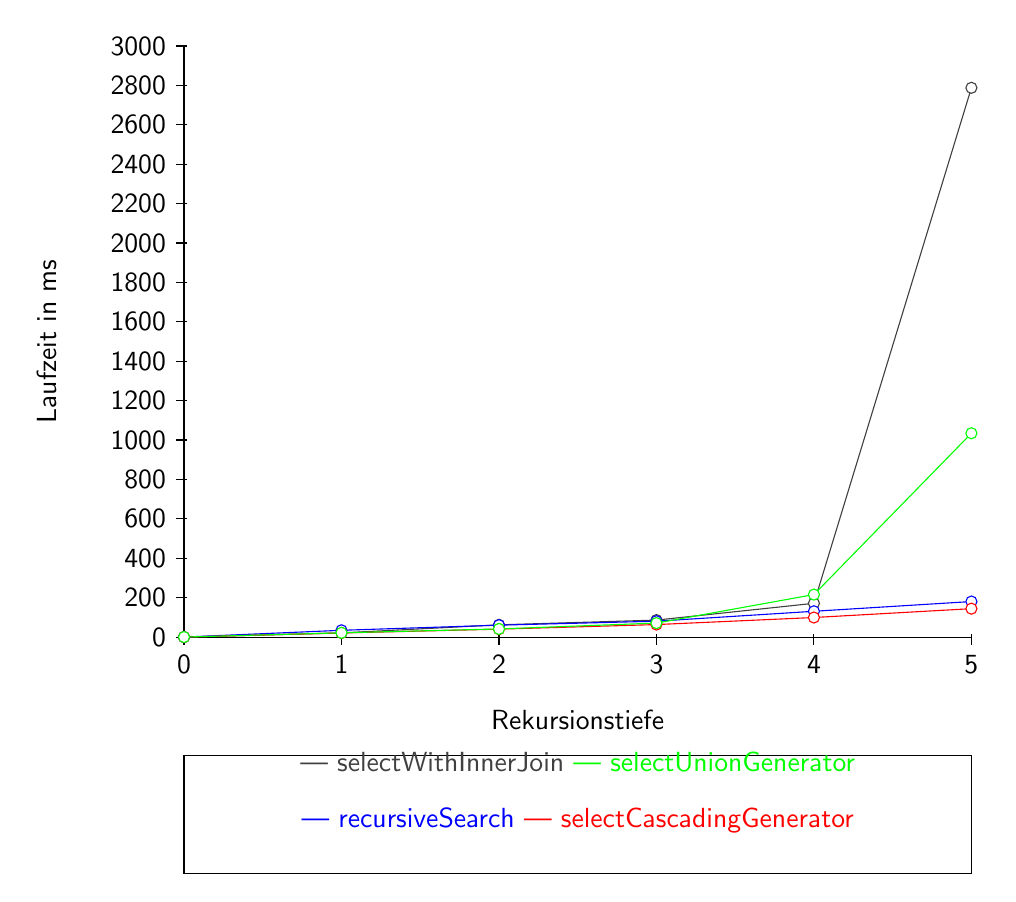
\begin{tikzpicture}[y=.0025cm, x=2cm,font=\sffamily]
	%axis
	\draw (0,0) -- coordinate (x axis mid) (5,0);
	\draw (0,0) -- coordinate (y axis mid) (0,3000);
	%ticks
	\foreach \x in {0,...,5}
	\draw (\x,1pt) -- (\x,-3pt)
	node[anchor=north] {\x};
	\foreach \y in {0,200,...,3000}
	\draw (1pt,\y) -- (-3pt,\y)
	node[anchor=east] {\y}; 
	%labels      
	\node[below=0.8cm] at (x axis mid) {Rekursionstiefe};
	\node[rotate=90, above=1.5cm] at (y axis mid) {Laufzeit in ms};
	%plots
	\draw[darkgray] plot[ mark=*, mark options={fill=white}] 
	coordinates{(0, 0)
		(1, 21.182)
		(2, 62.066)
		(3, 86.128)
		(4, 171.283)
		(5, 2787.659)
	};
	
	\draw[blue] plot[ mark=*, mark options={fill=white}] 
	coordinates{(0, 0)
		(1, 34.365)
		(2, 60.394)
		(3, 80.454)
		(4, 130.866)
		(5, 180.301)
	};
	\draw[red] plot[ mark=*, mark options={fill=white}] 
	coordinates{(0, 0)
		(1, 20.774)
		(2, 40.090)
		(3, 63.405)
		(4, 99.210)
		(5, 144.089)
	};
	\draw[green] plot[ mark=*, mark options={fill=white}] 
	coordinates{(0, 0)
		(1, 21.490)
		(2, 41.234)
		(3, 70.961)
		(4, 215.687)
		(5,1034.360)
	};
	
	\draw (0,-600) -- (5,-600) 
	(0,-600) -- (0,-1200)
	(0,-1200) -- (5,-1200)
	(5,-600) -- (5,-1200);
	\draw[draw=none] (0,0) -- (5,0) 
	node[draw=none, midway, yshift=-4.5em]
	{
		\textcolor{darkgray}{--- selectWithInnerJoin}
		\textcolor{green}{--- selectUnionGenerator} 
		
	};
	\draw[draw=none] (0,-600) -- (5,0) 
	node[draw=none, midway, yshift=-4.5em]
	{
		\textcolor{blue}{--- recursiveSearch} 
		\textcolor{red}{--- selectCascadingGenerator}
	};
	\end{tikzpicture}
	\caption{ relation\_wiki\_vote}
\end{figure}

\begin{table}[H]
	\begin{tabular}{l|l|l|l|l|l|}
		\cline{2-6}
		& \multicolumn{5}{|l|}{Laufzeit in MS}                                                                                                                                                  \\ \hline
		\multicolumn{1}{|l|}{\multirow{2}{2cm}{Rerkusions-tiefe}} & \multicolumn{2}{|l|}{\multirow{2}{3cm}{selectCascading Generator}} & \multirow{2}{2.8cm}{recursiveSearch} & \multirow{2}{2.5cm}{selectUnion Generator} & \multirow{2}{2.5cm}{selectInner JoinGenerator} \\
		\multicolumn{1}{|l|}{}
		& \multicolumn{2}{|l|}{}                                           &                                  &                                     &                                           \\ \hline
		
		\multicolumn{1}{|l|}{1}                                 & \multicolumn{2}{l|}{20.774}                                      & 34.365                                                & 21.490                                                    & 21.182                                                          \\ \hline
		\multicolumn{1}{|l|}{2}                                 & \multicolumn{2}{l|}{40.090}                                      & 60.394                                                & 41.234                                                    & 62.066                                                          \\ \hline
		\multicolumn{1}{|l|}{3}                                 & \multicolumn{2}{l|}{63.405}                                      & 80.454                                                & 70.961                                                    & 86.128                                                          \\ \hline
		\multicolumn{1}{|l|}{4}                                 & \multicolumn{2}{l|}{99.210}                                      & 130.866                                               & 215.687                                                   & 171.283                                                         \\ \hline
		\multicolumn{1}{|l|}{5}                                 & \multicolumn{2}{l|}{144.089}                                     & 180.301                                               & 1034.360                                                  & 2787.659                                                        \\ \hline
		
		
		
	\end{tabular}
	\caption{Laufzeit der SQLs für Tabelle relation\_wiki\_vote}
\end{table}

Bei den Wikipedia-Daten zeigt sich ein ähnliches Laufzeitverhalten wie bei den Epionions-Daten. InnerJoin und Standard-SQL verschlechtern sich von der vierten auf die fünfte Iterationsstufe massiv. Das verschachtelte Select weist hier über alle Rekursionsstufen die geringste Latenz auf.

\newpage

\paragraph{relation\_youtube}\mbox{}\\

\begin{figure}[H]
	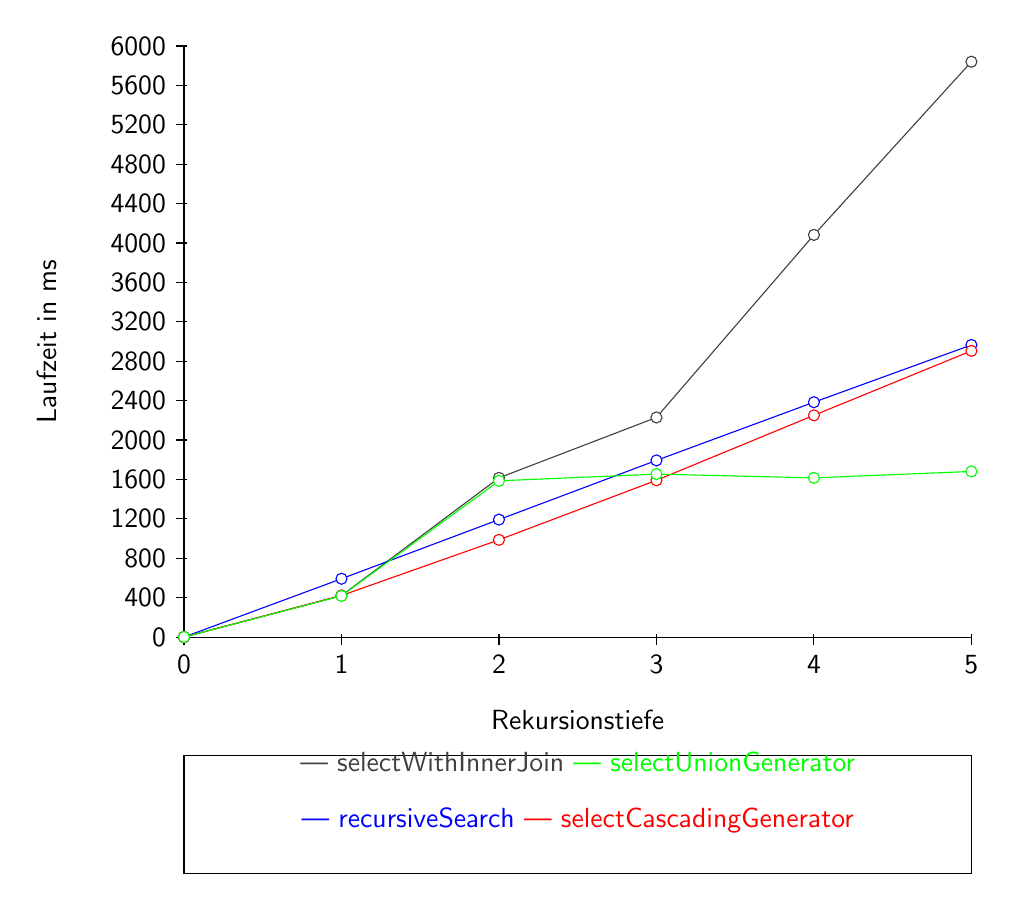
\begin{tikzpicture}[y=.00125cm, x=2cm,font=\sffamily]
	%axis
	\draw (0,0) -- coordinate (x axis mid) (5,0);
	\draw (0,0) -- coordinate (y axis mid) (0,6000);
	%ticks
	\foreach \x in {0,...,5}
	\draw (\x,1pt) -- (\x,-3pt)
	node[anchor=north] {\x};
	\foreach \y in {0,400,...,6000}
	\draw (1pt,\y) -- (-3pt,\y)
	node[anchor=east] {\y}; 
	%labels      
	\node[below=0.8cm] at (x axis mid) {Rekursionstiefe};
	\node[rotate=90, above=1.5cm] at (y axis mid) {Laufzeit in ms};
	%plots
	\draw[darkgray] plot[ mark=*, mark options={fill=white}] 
	coordinates{(0, 0)
		(1, 421.124)
		(2, 1615.843)
		(3, 2229.214)
		(4, 4082.179)
		(5, 5839.987)
	};
	
	\draw[blue] plot[ mark=*, mark options={fill=white}] 
	coordinates{(0, 0)
		(1, 592.063)
		(2, 1192.278)
		(3, 1793.281)
		(4, 2383.885)
		(5, 2964.950)
	};
	\draw[red] plot[ mark=*, mark options={fill=white}] 
	coordinates{(0, 0)
		(1, 421.464)
		(2, 986.995)
		(3, 1591.391)
		(4, 2250.832)
		(5, 2905.167)
	};
	\draw[green] plot[ mark=*, mark options={fill=white}] 
	coordinates{(0, 0)
		(1, 418.105)
		(2, 1585.836)
		(3, 1654.011)
		(4, 1615.986)
		(5, 1681.231)
	};
	
	\draw (0,-1200) -- (5,-1200) 
	(0,-1200) -- (0,-2400)
	(0,-2400) -- (5,-2400)
	(5,-1200) -- (5,-2400);
	\draw[draw=none] (0,0) -- (5,0) 
	node[draw=none, midway, yshift=-4.5em]
	{
		\textcolor{darkgray}{--- selectWithInnerJoin}
		\textcolor{green}{--- selectUnionGenerator} 
		
	};
	\draw[draw=none] (0,-1200) -- (5,0) 
	node[draw=none, midway, yshift=-4.5em]
	{
		\textcolor{blue}{--- recursiveSearch} 
		\textcolor{red}{--- selectCascadingGenerator}
	};
	\end{tikzpicture}
	\caption{ relation\_youtube}
\end{figure}

\begin{table}[H]
	\begin{tabular}{l|l|l|l|l|l|}
		\cline{2-6}
		& \multicolumn{5}{|l|}{Laufzeit in MS}                                                                                                                                                  \\ \hline
		\multicolumn{1}{|l|}{\multirow{2}{2cm}{Rerkusions-tiefe}} & \multicolumn{2}{|l|}{\multirow{2}{3cm}{selectCascading Generator}} & \multirow{2}{2.8cm}{recursiveSearch} & \multirow{2}{2.5cm}{selectUnion Generator} & \multirow{2}{2.5cm}{selectInner JoinGenerator} \\
		\multicolumn{1}{|l|}{}
		& \multicolumn{2}{|l|}{}                                           &                                  &                                     &                                           \\ \hline
		
		\multicolumn{1}{|l|}{1}                                 & \multicolumn{2}{l|}{421.464}                                     & 592.063                                               & 418.105                                                   & 421.124                                                         \\ \hline
		\multicolumn{1}{|l|}{2}                                 & \multicolumn{2}{l|}{986.995}                                     & 1192.278                                              & 1585.836                                                  & 1615.843                                                        \\ \hline
		\multicolumn{1}{|l|}{3}                                 & \multicolumn{2}{l|}{1591.391}                                    & 1793.281                                              & 1654.011                                                  & 2229.214                                                        \\ \hline
		\multicolumn{1}{|l|}{4}                                 & \multicolumn{2}{l|}{2250.832}                                    & 2383.885                                              & 1615.986                                                  & 4082.179                                                        \\ \hline
		\multicolumn{1}{|l|}{5}                                 & \multicolumn{2}{l|}{2905.167}                                    & 2964.950                                              & 1681.231                                                  & 5839.987                                                        \\ \hline
		
		
		
	\end{tabular}
	\caption{Laufzeit der SQLs für Tabelle relation\_youtube}
\end{table}

Bei den Youtube-Daten zeigen die Verschiedenen SQL-Statements ein sehr unterschiedliches Verhalten. Beim Standard-SQL gibt es einen deutlichen Anstieg zwischen von der ersten auf die zweite Rekursionstiefe. Für die weiteren Rekursionstiefen bleibt die Laufzeit dann ungefähr konstant. Das verschachtelte Select und die rekursive Funktion sind in ihrem Laufzeitverhalten sehr ähnlich. Beide steigen linear. Das InnerJoin zweigt bei steigender Rekursionstiefe das schlechteste Laufzeitverhalten.

\subsubsection{Antwortzeiten mit Indices}

Im Folgenden sind die Laufzeiten der SQL-Staments auf den Tabellen mit den Indices dargestellt.

\paragraph{relation\_epinions\_with\_index}\mbox{}\\

\begin{figure}[H]
	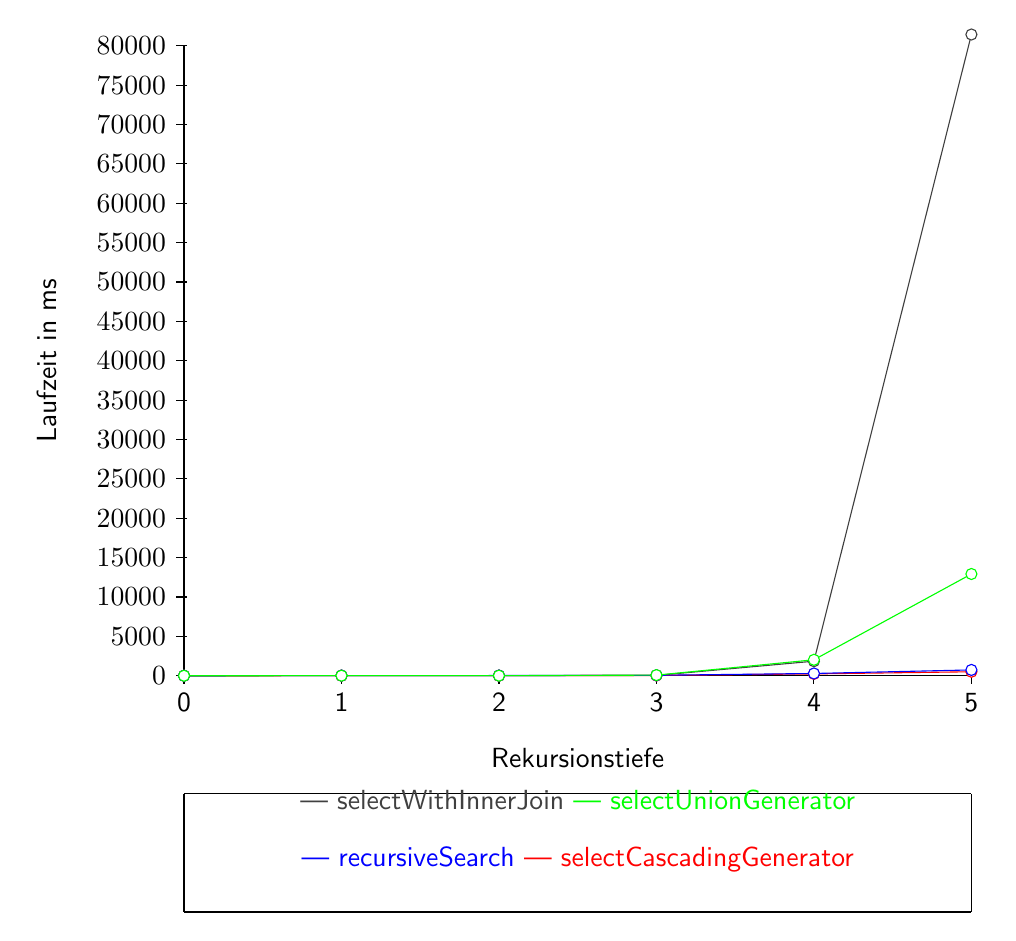
\begin{tikzpicture}[y=.5cm, x=2cm,font=\sffamily]
	%axis
	\draw (0,0) -- coordinate (x axis mid) (5,0);
	\draw (0,0) -- coordinate (y axis mid) (0,16);
	%ticks
	\foreach \x in {0,...,5}
	\draw (\x,1pt) -- (\x,-3pt)
	node[anchor=north] {\x};
	\foreach \y/\ytext in {
		0/0,
		1/5000,
		2/10000,
		3/15000,
		4/20000,
		5/25000,
		6/30000,
		7/35000,
		8/40000,
		9/45000,
		10/50000,
		11/55000,
		12/60000,
		13/65000,
		14/70000,
		15/75000,
		16/80000
	}
		\draw (1pt,\y) -- (-3pt,\y) node[anchor=east] {$\ytext$}; 
	%labels      
	\node[below=0.8cm] at (x axis mid) {Rekursionstiefe};
	\node[rotate=90, above=1.5cm] at (y axis mid) {Laufzeit in ms};
	%plots
	\draw[darkgray] plot[ mark=*, mark options={fill=white}] 
	coordinates{(0, 0)
		(1, 10.596/5000)
		(2, 10.739/5000)
		(3, 41.171/5000)
		(4, 0.3696)%1898.726/5000
		(5, 16.2872)%81436.561/5000
	};
	
	\draw[red] plot[ mark=*, mark options={fill=white}] 
	coordinates{(0, 0)
		(1, 8.231/5000)
		(2, 9.290/5000)
		(3, 36.244/5000)
		(4, 235.146/5000)
		(5, 504.793/5000)
	};
	\draw[blue] plot[ mark=*, mark options={fill=white}] 
	coordinates{(0, 0)
		(1, 18.999/5000)
		(2, 23.549/5000)
		(3, 54.953/5000)
		(4, 287.319/5000)
		(5, 737.300/5000)
	};
	\draw[green] plot[ mark=*, mark options={fill=white}] 
	coordinates{(0, 0)
		(1, 8.855/5000)
		(2, 10.304/5000)
		(3, 78.303/5000)
		(4, 2024.069/5000)
		(5, 12920.747/5000)
	};
	\draw (0,-3) -- (5,-3) 
(0,-3) -- (0,-6)
(0,-6) -- (5,-6)
(5,-3) -- (5,-6);
\draw[draw=none] (0,0) -- (5,0) 
node[draw=none, midway, yshift=-4.5em]
{
	\textcolor{darkgray}{--- selectWithInnerJoin}
	\textcolor{green}{--- selectUnionGenerator} 
	
};
\draw[draw=none] (0,-3) -- (5,0) 
node[draw=none, midway, yshift=-4.5em]
{
	\textcolor{blue}{--- recursiveSearch} 
	\textcolor{red}{--- selectCascadingGenerator}
};
	\end{tikzpicture}
	\caption{ relation\_epinions\_with\_index}
\end{figure}

\begin{table}[H]
	\centering
	\begin{tabular}{l|l|l|l|l|l|}
		\cline{2-6}
		& \multicolumn{5}{|l|}{Laufzeit in MS}                                                                                                                                                  \\ \hline
		\multicolumn{1}{|l|}{\multirow{2}{2cm}{Rerkusions-tiefe}} & \multicolumn{2}{|l|}{\multirow{2}{3cm}{selectCascading Generator}} & \multirow{2}{2.8cm}{recursiveSearch} & \multirow{2}{2.5cm}{selectUnion Generator} & \multirow{2}{2.5cm}{selectInner JoinGenerator} \\
		\multicolumn{1}{|l|}{}
		& \multicolumn{2}{|l|}{}                                           &                                  &                                     &                                           \\ \hline
		
		
\multicolumn{1}{|l|}{1}                                 & \multicolumn{2}{l|}{8.231}                                       & 18.999                                                & 8.885                                                     & 10.596                                                          \\ \hline
\multicolumn{1}{|l|}{2}                                 & \multicolumn{2}{l|}{9.290}                                       & 23.549                                                & 10.304                                                    & 10.739                                                          \\ \hline
\multicolumn{1}{|l|}{3}                                 & \multicolumn{2}{l|}{36.244}                                      & 54.953                                                & 78.303                                                    & 41.171                                                          \\ \hline
\multicolumn{1}{|l|}{4}                                 & \multicolumn{2}{l|}{235.146}                                     & 287.319                                               & 2024.069                                                  & 1898.726                                                        \\ \hline
\multicolumn{1}{|l|}{5}                                 & \multicolumn{2}{l|}{504.793}                                     & 737.300                                               & 12920.747                                                 & 81436.561                                                       \\ \hline

	\end{tabular}
	\caption{Laufzeit der SQLs für Tabelle relation\_epinions\_with\_index}
\end{table}

Bei den Epinions-Daten wirkt sich das Einführen der Indices gering aus. Beim innerJoin ist praktisch kein Unterschied zu messbar. Beim StandardSQL führte es sogar zu einer deutlichen Verschlechterung in der fünften Rekursionstufe. Beim verschachtelten Select und bei der rekursieven Funktion gab es eine Verbesserung, diese viel jedoch verhältnismäßig gering aus. Im besten Fall verbesserte sich die fünfte Rekursionstufe von 677 Millisekunden auf 505 Millisekunden.

\paragraph{relation\_livejournal\_with\_index}\mbox{}\\
\begin{figure}[H]
	
	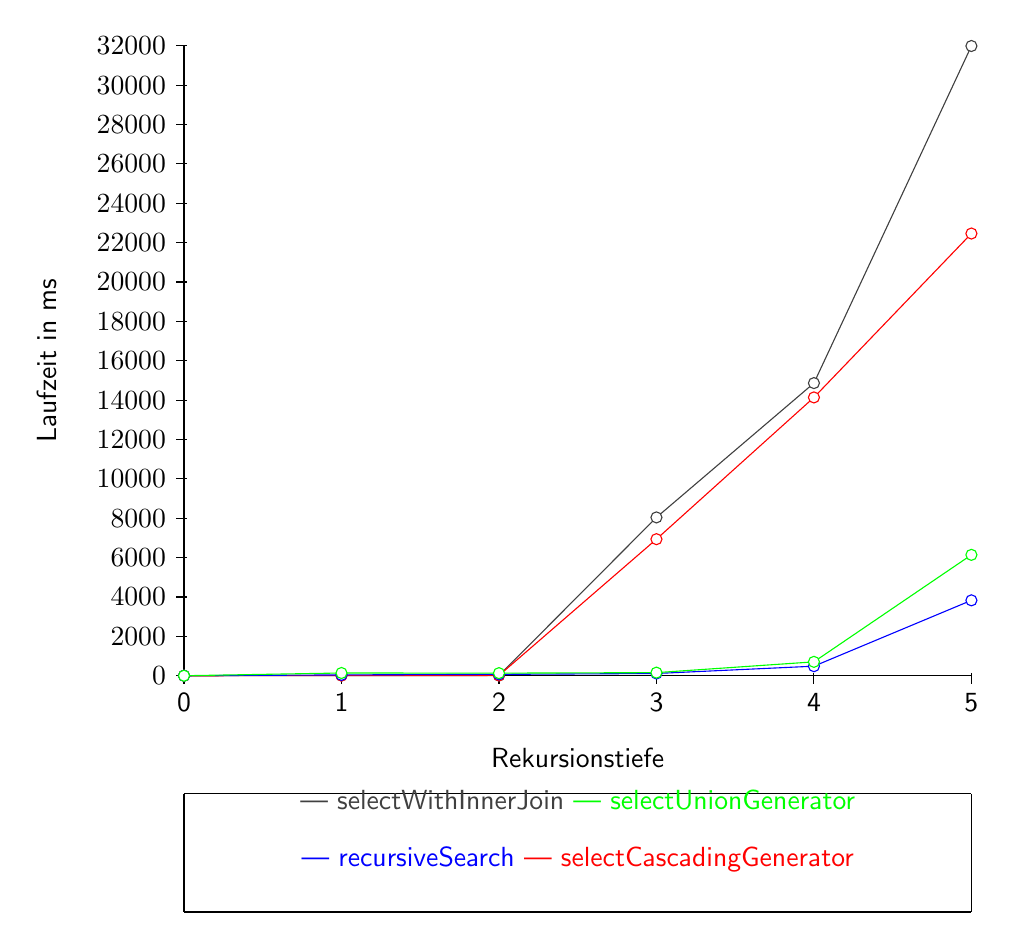
\begin{tikzpicture}[y=.5cm, x=2cm,font=\sffamily]
	%axis
	\draw (0,0) -- coordinate (x axis mid) (5,0);
	\draw (0,0) -- coordinate (y axis mid) (0,16);
	%ticks
	\foreach \x in {0,...,5}
	\draw (\x,1pt) -- (\x,-3pt)
	node[anchor=north] {\x};
	\foreach \y/\ytext in {
		0/0,
		1/2000,
		2/4000,
		3/6000,
		4/8000,
		5/10000,
		6/12000,
		7/14000,
		8/16000,
		9/18000,
		10/20000,
		11/22000,
		12/24000,
		13/26000,
		14/28000,
		15/30000,
		16/32000,
	}
	\draw (1pt,\y) -- (-3pt,\y) node[anchor=east] {$\ytext$};
	%labels      
	\node[below=0.8cm] at (x axis mid) {Rekursionstiefe};
	\node[rotate=90, above=1.5cm] at (y axis mid) {Laufzeit in ms};
	%plots
	
	\draw[darkgray] plot[mark=*, mark options={fill=white}] 
	coordinates{(0, 0)
		(1, 9.165/2000)
		(2,	11.862/2000)
		(3, 8042.794/2000)
		(4, 14865.814/2000)
		(5,	 15.995)%31990.436/2000)
	};	
	\draw[red] plot[mark=*, mark options={fill=white}] 
	coordinates{(0, 0)
		(1, 0.004)%8.672/2000
		(2,	15.240/2000)
		(3, 6936.935/2000)
		(4, 14137.544/2000)%
		(5,	11.232)%22464.363/2000	
	};
	\draw[blue] plot[mark=*, mark options={fill=white}] 
	coordinates{(0, 0)
		(1, 42.010/2000)
		(2,	69.129/2000)
		(3, 114.466/2000)
		(4, 484.914/2000)
		(5,	3830.355/2000)
	};
	\draw[green] plot[mark=*, mark options={fill=white}] 
	coordinates{(0, 0)
		(1, 139.294/2000)
		(2,	131.623/2000)
		(3, 157.707/2000)
		(4, 705.293/2000)
		(5, 6140.824/2000)
	};
	\draw (0,-3) -- (5,-3) 
(0,-3) -- (0,-6)
(0,-6) -- (5,-6)
(5,-3) -- (5,-6);
\draw[draw=none] (0,0) -- (5,0) 
node[draw=none, midway, yshift=-4.5em]
{
	\textcolor{darkgray}{--- selectWithInnerJoin}
	\textcolor{green}{--- selectUnionGenerator} 
	
};
\draw[draw=none] (0,-3) -- (5,0) 
node[draw=none, midway, yshift=-4.5em]
{
	\textcolor{blue}{--- recursiveSearch} 
	\textcolor{red}{--- selectCascadingGenerator}
};
	\end{tikzpicture}
	\caption{ relation\_livejournal\_with\_index}
\end{figure}

\begin{table}[H]
	\centering
	\begin{tabular}{l|l|l|l|l|l|}
		\cline{2-6}
		& \multicolumn{5}{|l|}{Laufzeit in MS}                                                                                                                                                  \\ \hline
		\multicolumn{1}{|l|}{\multirow{2}{2cm}{Rerkusions-tiefe}} & \multicolumn{2}{|l|}{\multirow{2}{3cm}{selectCascading Generator}} & \multirow{2}{2.8cm}{recursiveSearch} & \multirow{2}{2.5cm}{selectUnion Generator} & \multirow{2}{2.5cm}{selectInner JoinGenerator} \\
		\multicolumn{1}{|l|}{}
		& \multicolumn{2}{|l|}{}                                           &                                  &                                     &                                           \\ \hline
		
		
		\multicolumn{1}{|l|}{1}                                 & \multicolumn{2}{l|}{8.672}                                       & 42.010                                                & 139.294                                                   & 9.165                                                           \\ \hline
		\multicolumn{1}{|l|}{2}                                 & \multicolumn{2}{l|}{15.240}                                      & 69.129                                                & 131.623                                                   & 11.862                                                          \\ \hline
		\multicolumn{1}{|l|}{3}                                 & \multicolumn{2}{l|}{6936.935}                                    & 114.466                                               & 157.707                                                   & 8042.794                                                        \\ \hline
		\multicolumn{1}{|l|}{4}                                 & \multicolumn{2}{l|}{14137.544}                                   & 484.914                                               & 705.293                                                   & 14865.814                                                       \\ \hline
		\multicolumn{1}{|l|}{5}                                 & \multicolumn{2}{l|}{22464.363}                                   & 3830.355                                              & 6140.824                                                  & 31990.436                                                       \\ \hline
	\end{tabular}
	\caption{Laufzeit der SQLs für Tabelle relation\_livejournal\_with\_index}
\end{table}
Die Verwendung der Indices führt zu einer erheblich besseren Latenz. Die Laufzeit in der ersten Rekursionsstufe verbessert sich von von mindestens 4,7 Sekunden auf im besten Fall 8.7 Millisekunden. Auch in der fünften Rekursionsstufe verkürtzt sich die Laufzeit deutlich.

\paragraph{relation\_facebook\_with\_index}\mbox{}\\

\begin{figure}[H]
	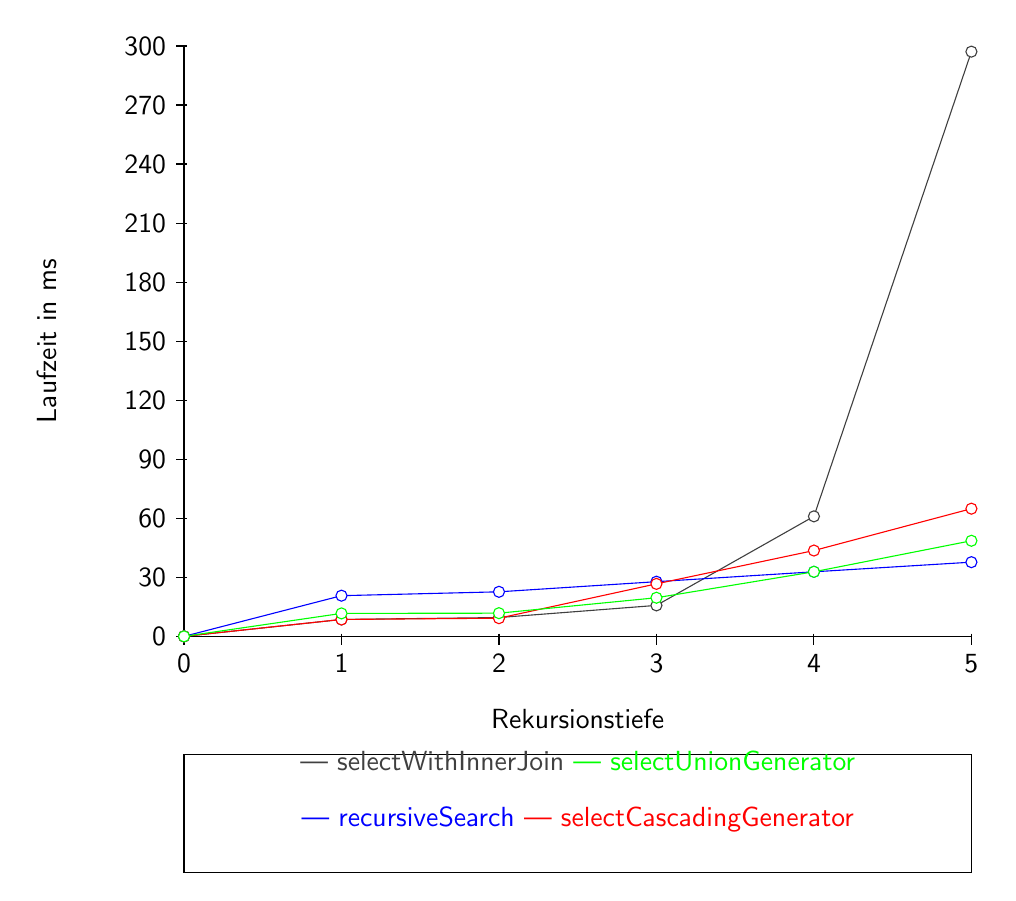
\begin{tikzpicture}[y=.025cm, x=2cm,font=\sffamily]
	%axis
	\draw (0,0) -- coordinate (x axis mid) (5,0);
	\draw (0,0) -- coordinate (y axis mid) (0,300);
	%ticks
	\foreach \x in {0,...,5}
	\draw (\x,1pt) -- (\x,-3pt)
	node[anchor=north] {\x};
	\foreach \y in {0,30,...,300}
	\draw (1pt,\y) -- (-3pt,\y)
	node[anchor=east] {\y}; 
	%labels      
	\node[below=0.8cm] at (x axis mid) {Rekursionstiefe};
	\node[rotate=90, above=1.5cm] at (y axis mid) {Laufzeit in ms};
	%plots
	\draw[darkgray] plot[ mark=*, mark options={fill=white}] 
	coordinates{(0, 0)
		(1, 8.585)
		(2, 9.565)
		(3, 15.738)
		(4, 60.976)
		(5, 297.115)
	};
	
	\draw[blue] plot[ mark=*, mark options={fill=white}] 
	coordinates{(0, 0)
		(1, 20.674)
		(2, 22.639)
		(3, 27.788)
		(4, 32.804)
		(5, 37.706)
	};
	\draw[red] plot[ mark=*, mark options={fill=white}] 
	coordinates{(0, 0)
		(1, 8.594)
		(2, 9.239)
		(3, 26.683)
		(4, 43.610)
		(5, 64.882)
	};
	\draw[green] plot[ mark=*, mark options={fill=white}] 
	coordinates{(0, 0)
		(1, 11.672)
		(2, 11.787)
		(3, 19.625)
		(4, 32.817)
		(5, 48.580)
	};
	
	\draw (0,-60) -- (5,-60) 
	(0,-60) -- (0,-120)
	(0,-120) -- (5,-120)
	(5,-60) -- (5,-120);
	\draw[draw=none] (0,0) -- (5,0) 
	node[draw=none, midway, yshift=-4.5em]
	{
		\textcolor{darkgray}{--- selectWithInnerJoin}
		\textcolor{green}{--- selectUnionGenerator} 
		
	};
	\draw[draw=none] (0,-60) -- (5,0) 
	node[draw=none, midway, yshift=-4.5em]
	{
		\textcolor{blue}{--- recursiveSearch} 
		\textcolor{red}{--- selectCascadingGenerator}
	};
	\end{tikzpicture}
	\caption{ relation\_facebook\_with\_index}
\end{figure}

\begin{table}[H]
	\centering
	\begin{tabular}{l|l|l|l|l|l|}
		\cline{2-6}
		& \multicolumn{5}{|l|}{Laufzeit in MS}                                                                                                                                                  \\ \hline
		\multicolumn{1}{|l|}{\multirow{2}{2cm}{Rerkusions-tiefe}} & \multicolumn{2}{|l|}{\multirow{2}{3cm}{selectCascading Generator}} & \multirow{2}{2.8cm}{recursiveSearch} & \multirow{2}{2.5cm}{selectUnion Generator} & \multirow{2}{2.5cm}{selectInner JoinGenerator} \\
		\multicolumn{1}{|l|}{}
		& \multicolumn{2}{|l|}{}                                           &                                  &                                     &                                           \\ \hline
		
		\multicolumn{1}{|l|}{1}                                 & \multicolumn{2}{l|}{8.594}                                       & 20.674                                                & 11.672                                                    & 8.585                                                           \\ \hline
		\multicolumn{1}{|l|}{2}                                 & \multicolumn{2}{l|}{9.239}                                       & 22.639                                                & 11.787                                                    & 9.565                                                           \\ \hline
		\multicolumn{1}{|l|}{3}                                 & \multicolumn{2}{l|}{26.683}                                      & 27.788                                                & 19.625                                                    & 15.738                                                          \\ \hline
		\multicolumn{1}{|l|}{4}                                 & \multicolumn{2}{l|}{43.610}                                      & 32.804                                                & 32.817                                                    & 60.976                                                              \\ \hline
		\multicolumn{1}{|l|}{5}                                 & \multicolumn{2}{l|}{64.882}                                      & 37.706                                                & 48.580                                                    & 297.115                                                         \\ \hline
	\end{tabular}
	\caption{Laufzeit der SQLs für Tabelle relation\_facebook\_with\_index}
\end{table}

Bei den Facebook Daten lässt sich durch die Indices in fast allen Fällen eine Verbesserung der Latenz erreichen. Außnahme ist hier der InnerJoin, hier ist keine wirkliche Verbesserung erkannbar. In der fünften Rekursionsstufe liegt die Latenz im besten Fall bei 38 Millisekunden mit der rekursiven Funktion. Ohne Indices liegt dieser Wert bei 89 Millisekunden und wird durch das verschachtelte SQL erreicht. 

\paragraph{relation\_wiki\_vote\_with\_index}\mbox{}\\

\begin{figure}[H]
	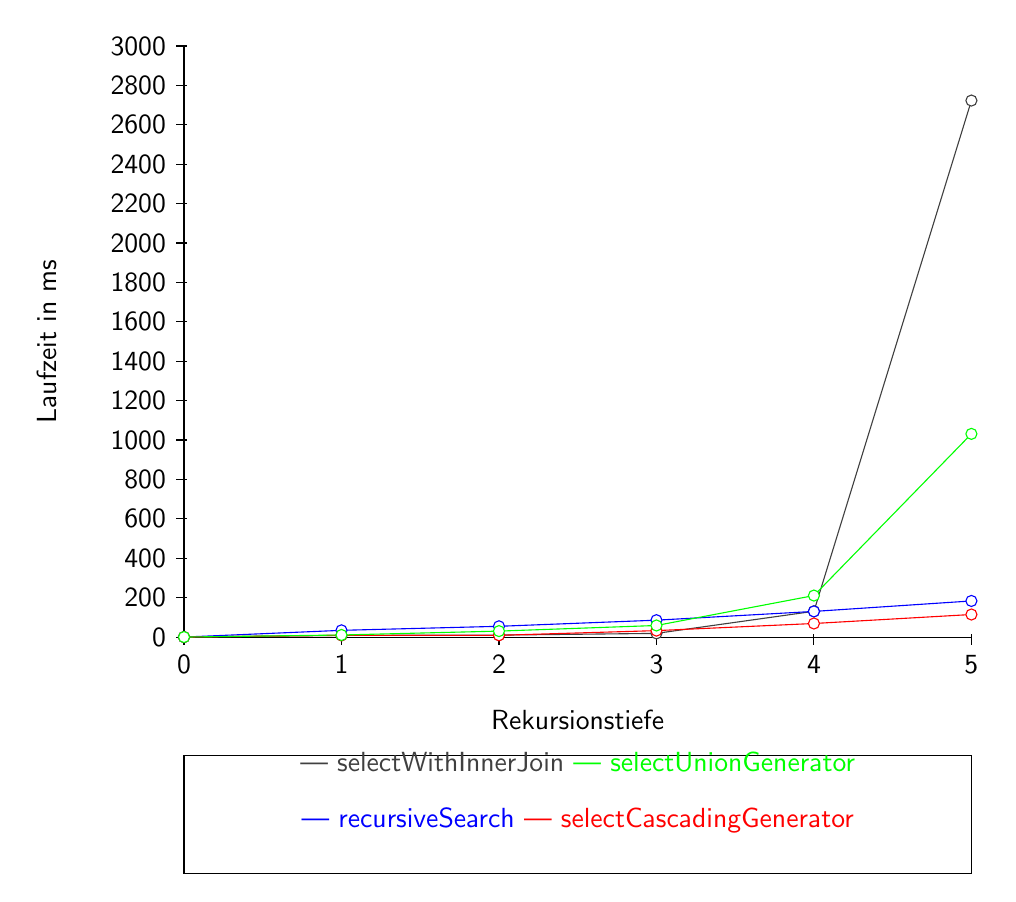
\begin{tikzpicture}[y=.0025cm, x=2cm,font=\sffamily]
	%axis
	\draw (0,0) -- coordinate (x axis mid) (5,0);
	\draw (0,0) -- coordinate (y axis mid) (0,3000);
	%ticks
	\foreach \x in {0,...,5}
	\draw (\x,1pt) -- (\x,-3pt)
	node[anchor=north] {\x};
	\foreach \y in {0,200,...,3000}
	\draw (1pt,\y) -- (-3pt,\y)
	node[anchor=east] {\y}; 
	%labels      
	\node[below=0.8cm] at (x axis mid) {Rekursionstiefe};
	\node[rotate=90, above=1.5cm] at (y axis mid) {Laufzeit in ms};
	%plots
	\draw[darkgray] plot[ mark=*, mark options={fill=white}] 
	coordinates{(0, 0)
		(1, 8.481)
		(2, 9.903)
		(3, 18.657)
		(4, 130.842)
		(5, 2722.908)
	};
	
	\draw[blue] plot[ mark=*, mark options={fill=white}] 
	coordinates{(0, 0)
		(1, 34.144)
		(2, 54.617)
		(3, 85.721)
		(4, 130.150)
		(5, 183.301)
	};
	\draw[red] plot[ mark=*, mark options={fill=white}] 
	coordinates{(0, 0)
		(1, 8.716)
		(2, 8.868)
		(3, 32.682)
		(4, 68.856)
		(5, 114.462)
	};
	\draw[green] plot[ mark=*, mark options={fill=white}] 
	coordinates{(0, 0)
		(1, 10.474)
		(2, 30.212)
		(3, 58.762)
		(4, 210.655)
		(5, 1031.234)
	};
	
	\draw (0,-600) -- (5,-600) 
	(0,-600) -- (0,-1200)
	(0,-1200) -- (5,-1200)
	(5,-600) -- (5,-1200);
	\draw[draw=none] (0,0) -- (5,0) 
	node[draw=none, midway, yshift=-4.5em]
	{
		\textcolor{darkgray}{--- selectWithInnerJoin}
		\textcolor{green}{--- selectUnionGenerator} 
		
	};
	\draw[draw=none] (0,-600) -- (5,0) 
	node[draw=none, midway, yshift=-4.5em]
	{
		\textcolor{blue}{--- recursiveSearch} 
		\textcolor{red}{--- selectCascadingGenerator}
	};
	\end{tikzpicture}
	\caption{ relation\_wiki\_vote}
\end{figure}



\begin{table}[H]
	\centering
	\begin{tabular}{l|l|l|l|l|l|}
		\cline{2-6}
		& \multicolumn{5}{|l|}{Laufzeit in MS}                                                                                                                                                  \\ \hline
		\multicolumn{1}{|l|}{\multirow{2}{2cm}{Rerkusions-tiefe}} & \multicolumn{2}{|l|}{\multirow{2}{3cm}{selectCascading Generator}} & \multirow{2}{2.8cm}{recursiveSearch} & \multirow{2}{2.5cm}{selectUnion Generator} & \multirow{2}{2.5cm}{selectInner JoinGenerator} \\
		\multicolumn{1}{|l|}{}
		& \multicolumn{2}{|l|}{}                                           &                                  &                                     &                                           \\ \hline
		
	\multicolumn{1}{|l|}{1}                                 & \multicolumn{2}{l|}{8.716}                                       & 34.144                                                & 10.474                                                    & 8.481                                                           \\ \hline
	\multicolumn{1}{|l|}{2}                                 & \multicolumn{2}{l|}{8.868}                                       & 54.617                                                & 30.212                                                    & 9.903                                                           \\ \hline
	\multicolumn{1}{|l|}{3}                                 & \multicolumn{2}{l|}{32.682}                                      & 85.721                                                & 58.762                                                    & 18.657                                                          \\ \hline
	\multicolumn{1}{|l|}{4}                                 & \multicolumn{2}{l|}{68.856}                                      & 130.150                                               & 210.655                                                   & 130.842                                                         \\ \hline
	\multicolumn{1}{|l|}{5}                                 & \multicolumn{2}{l|}{114.462}                                     & 183.301                                               & 1031.234                                                  & 2722.908                                                        \\ \hline
	
	\end{tabular}
	\caption{Laufzeit der SQLs für Tabelle relation\_wiki\_vote\_with\_index}
\end{table}

Das Einführen der Indices hat eine vergleichsweise geringe Wirkung auf die Laufzeiten der verschienden SQLs. Zwar gibt es realativ gesehen deutliche Verbesserungen in den ersten beiden Rekursionsstufen. In der fünften Rekursionsstufe  verbessert sich jedoch nur das verschachtelte Select um knapp 21\% gegenüber der Tabelle ohne Indices. Für die anderen Statements ergaben sich hier keine Verbesserungen.

\paragraph{relation\_youtube\_with\_index}\mbox{}\\

\begin{figure}[H]
	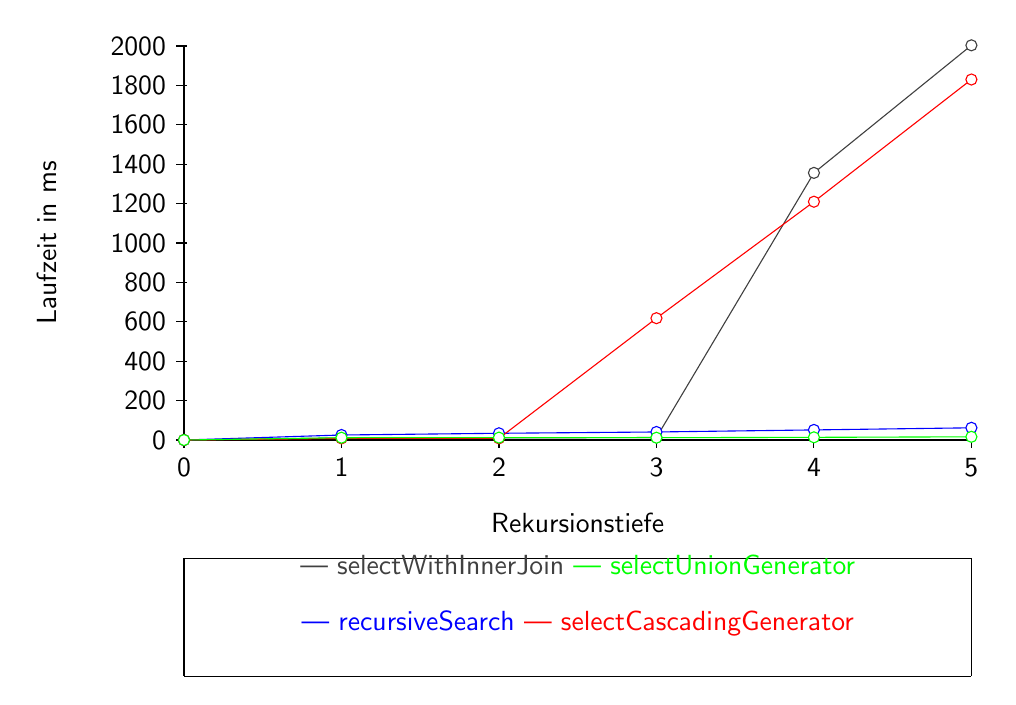
\begin{tikzpicture}[y=.0025cm, x=2cm,font=\sffamily]
	%axis
	\draw (0,0) -- coordinate (x axis mid) (5,0);
	\draw (0,0) -- coordinate (y axis mid) (0,2000);
	%ticks
	\foreach \x in {0,...,5}
	\draw (\x,1pt) -- (\x,-3pt)
	node[anchor=north] {\x};
	\foreach \y in {0,200,...,2000}
	\draw (1pt,\y) -- (-3pt,\y)
	node[anchor=east] {\y}; 
	%labels      
	\node[below=0.8cm] at (x axis mid) {Rekursionstiefe};
	\node[rotate=90, above=1.5cm] at (y axis mid) {Laufzeit in ms};
	%plots
	\draw[darkgray] plot[ mark=*, mark options={fill=white}] 
	coordinates{(0, 0)
		(1, 10.213)
		(2, 10.587)
		(3, 12.858)
		(4, 1355.866)
		(5, 2003.275)
	};
	
	\draw[blue] plot[ mark=*, mark options={fill=white}] 
	coordinates{(0, 0)
		(1, 25.508)
		(2, 34.273)
		(3, 40.852)
		(4, 51.285)
		(5, 62.037)
	};
	\draw[red] plot[ mark=*, mark options={fill=white}] 
	coordinates{(0, 0)
		(1, 8.370)
		(2, 8.528)
		(3, 618.336)
		(4, 1209.513)
		(5, 1829.757)
	};
	\draw[green] plot[ mark=*, mark options={fill=white}] 
	coordinates{(0, 0)
		(1, 11.801)
		(2, 12.265)
		(3, 11.832)
		(4, 13.644)
		(5, 16.362)
	};
	
	\draw (0,-600) -- (5,-600) 
	(0,-600) -- (0,-1200)
	(0,-1200) -- (5,-1200)
	(5,-600) -- (5,-1200);
	\draw[draw=none] (0,0) -- (5,0) 
	node[draw=none, midway, yshift=-4.5em]
	{
		\textcolor{darkgray}{--- selectWithInnerJoin}
		\textcolor{green}{--- selectUnionGenerator} 
		
	};
	\draw[draw=none] (0,-600) -- (5,0) 
	node[draw=none, midway, yshift=-4.5em]
	{
		\textcolor{blue}{--- recursiveSearch} 
		\textcolor{red}{--- selectCascadingGenerator}
	};
	\end{tikzpicture}
	\caption{ relation\_youtube\_with\_index}
\end{figure}

\begin{table}[H]
	\centering
	\begin{tabular}{l|l|l|l|l|l|}
		\cline{2-6}
		& \multicolumn{5}{|l|}{Laufzeit in MS}                                                                                                                                                  \\ \hline
		\multicolumn{1}{|l|}{\multirow{2}{2cm}{Rerkusions-tiefe}} & \multicolumn{2}{|l|}{\multirow{2}{3cm}{selectCascading Generator}} & \multirow{2}{2.8cm}{recursiveSearch} & \multirow{2}{2.5cm}{selectUnion Generator} & \multirow{2}{2.5cm}{selectInner JoinGenerator} \\
		\multicolumn{1}{|l|}{}
		& \multicolumn{2}{|l|}{}                                           &                                  &                                     &                                           \\ \hline
		
		\multicolumn{1}{|l|}{1}                                 & \multicolumn{2}{l|}{8.370}                                       & 25.508                                                & 11.801                                                    & 10.213                                                          \\ \hline
		\multicolumn{1}{|l|}{2}                                 & \multicolumn{2}{l|}{8.528}                                       & 34.273                                                & 12.265                                                    & 10.587                                                          \\ \hline
		\multicolumn{1}{|l|}{3}                                 & \multicolumn{2}{l|}{618.336}                                     & 40.852                                                & 11.832                                                    & 12.858                                                          \\ \hline
		\multicolumn{1}{|l|}{4}                                 & \multicolumn{2}{l|}{1209.513}                                    & 51.285                                                & 13.644                                                    & 1355.866                                                        \\ \hline
		\multicolumn{1}{|l|}{5}                                 & \multicolumn{2}{l|}{1829.757}                                    & 62.037                                                & 16.362                                                    & 2003.275                                                        \\ \hline
		
		
	\end{tabular}
	\caption{Laufzeit der SQLs für Tabelle relation\_youtube\_with\_index}
\end{table}

Die Verwendung von Indices zeigt sich eine deutliche Verbesserung der Laufzeiten. Alle Statements weißen eine deutlich geringere Latenz auf. Die größte Veränderung zeigt hierbei das Standard-SQL Statement. Hier verringert sich die Latenz von 1,6 Sekunden auf 16 Millisekunden. Auch die Laufzeit der rekursiven Funktion verbessert sich von knapp 3 Sekunden auf 62 Millisekunden deutlich. 

\subsubsection{Antwortzeiten mit partitionierten Tabellen und Indices}
Im Folgenden sind die Laufzeiten der SQL-Statements auf den partitionierten Tabellen dargestellt.
\paragraph{relation\_epinions\_partitioned}\mbox{}\\

\begin{figure}[H]
	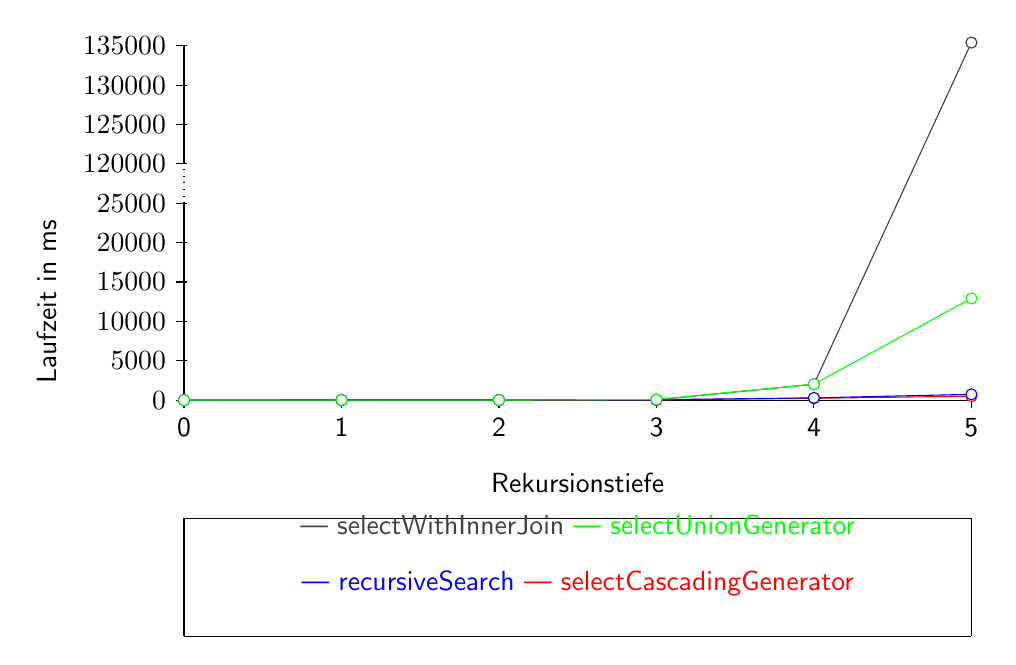
\begin{tikzpicture}[y=.5cm, x=2cm,font=\sffamily]
	%axis
	\draw (0,0) -- coordinate (x axis mid) (5,0);
	\draw (0,0) -- coordinate (y axis mid) (0,5);
	\draw[dotted] (0,5) -- (0,6);
	\draw (0,6) -- (0,9);
	%ticks
	\foreach \x in {0,...,5}
	\draw (\x,1pt) -- (\x,-3pt)
	node[anchor=north] {\x};
		\foreach \y/\ytext in {
		0/0,
		1/5000,
		2/10000,
		3/15000,
		4/20000,
		5/25000,
		6/120000,
		7/125000,
		8/130000,
		9/135000
	}
	\draw (1pt,\y) -- (-3pt,\y) node[anchor=east] {$\ytext$};
	%labels      
	\node[below=0.8cm] at (x axis mid) {Rekursionstiefe};
	\node[rotate=90, above=1.5cm] at (y axis mid) {Laufzeit in ms};
	%plots
	\draw[darkgray] plot[ mark=*, mark options={fill=white}] 
	coordinates{(0, 0)
		(1, 0.002)%8.846/5000)
		(2, 0.002)%9.924/5000)
		(3, 43.439/5000)
		(4, 2021.028/5000)
		(5, 9.082)%136242.608/15000)
	};
	
	\draw[red] plot[ mark=*, mark options={fill=white}] 
	coordinates{(0, 0)
		(1, 0.002)%8.231/5000)
		(2, 0.002)%9.290/5000)
		(3, 36.244/5000)
		(4, 235.146/5000)
		(5, 504.793/5000)
	};
	\draw[blue] plot[ mark=*, mark options={fill=white}] 
	coordinates{(0, 0)
		(1, 18.999/5000)
		(2, 23.549/5000)
		(3, 54.953/5000)
		(4, 287.319/5000)
		(5, 737.300/5000)
	};
	\draw[green] plot[ mark=*, mark options={fill=white}] 
	coordinates{(0, 0)
		(1, 8.855/5000)
		(2, 10.304/5000)
		(3, 78.303/5000)
		(4,2024.069/5000)
		(5,12920.747/5000)
	};
\draw (0,-3) -- (5,-3) 
(0,-3) -- (0,-6)
(0,-6) -- (5,-6)
(5,-3) -- (5,-6);
\draw[draw=none] (0,0) -- (5,0) 
node[draw=none, midway, yshift=-4.5em]
{
	\textcolor{darkgray}{--- selectWithInnerJoin}
	\textcolor{green}{--- selectUnionGenerator} 
	
};
\draw[draw=none] (0,-3) -- (5,0) 
node[draw=none, midway, yshift=-4.5em]
{
	\textcolor{blue}{--- recursiveSearch} 
	\textcolor{red}{--- selectCascadingGenerator}
};
	\end{tikzpicture}
	\caption{ relation\_epinions\_partitioned}
\end{figure}

\begin{table}[H]
	\centering
	\begin{tabular}{l|l|l|l|l|l|}
		\cline{2-6}
		& \multicolumn{5}{|l|}{Laufzeit in MS}                                                                                                                                                  \\ \hline
		\multicolumn{1}{|l|}{\multirow{2}{2cm}{Rerkusions-tiefe}} & \multicolumn{2}{|l|}{\multirow{2}{3cm}{selectCascading Generator}} & \multirow{2}{2.8cm}{recursiveSearch} & \multirow{2}{2.5cm}{selectUnion Generator} & \multirow{2}{2.5cm}{selectInner JoinGenerator} \\
		\multicolumn{1}{|l|}{}
		& \multicolumn{2}{|l|}{}                                           &                                  &                                     &                                           \\ \hline
		
	\multicolumn{1}{|l|}{1}                                 & \multicolumn{2}{l|}{8.231}                                       & 18.999                                                & 8.855                                                     & 8.846                                                           \\ \hline
	\multicolumn{1}{|l|}{2}                                 & \multicolumn{2}{l|}{9.290}                                       & 23.549                                                & 10.304                                                    & 9.924                                                           \\ \hline
	\multicolumn{1}{|l|}{3}                                 & \multicolumn{2}{l|}{36.244}                                      & 54.953                                                & 78.303                                                    & 43.439                                                          \\ \hline
	\multicolumn{1}{|l|}{4}                                 & \multicolumn{2}{l|}{235.146}                                     & 287.319                                               & 2024.069                                                  & 2021.028                                                        \\ \hline
	\multicolumn{1}{|l|}{5}                                 & \multicolumn{2}{l|}{504.793}                                     & 737.300                                               & 12920.747                                                 & 136242.608                                                      \\ \hline
	
		
		
	\end{tabular}
	\caption{Laufzeit der SQLs für Tabelle relation\_epinions\_partitioned}
\end{table}

Durch die Partitionierung der Tabelle ergeben sich keine Verbesserungen in der Latenz. Das gilt für alle Statements. Die Laufzeit beim InnerJoin verschlechtert sich sogar deutlich gegenüber der Tabelle bei der nur Indices verwendet wurden.

\paragraph{relation\_livejournal\_partitioned}\mbox{}\\
\begin{figure}[H]
	
	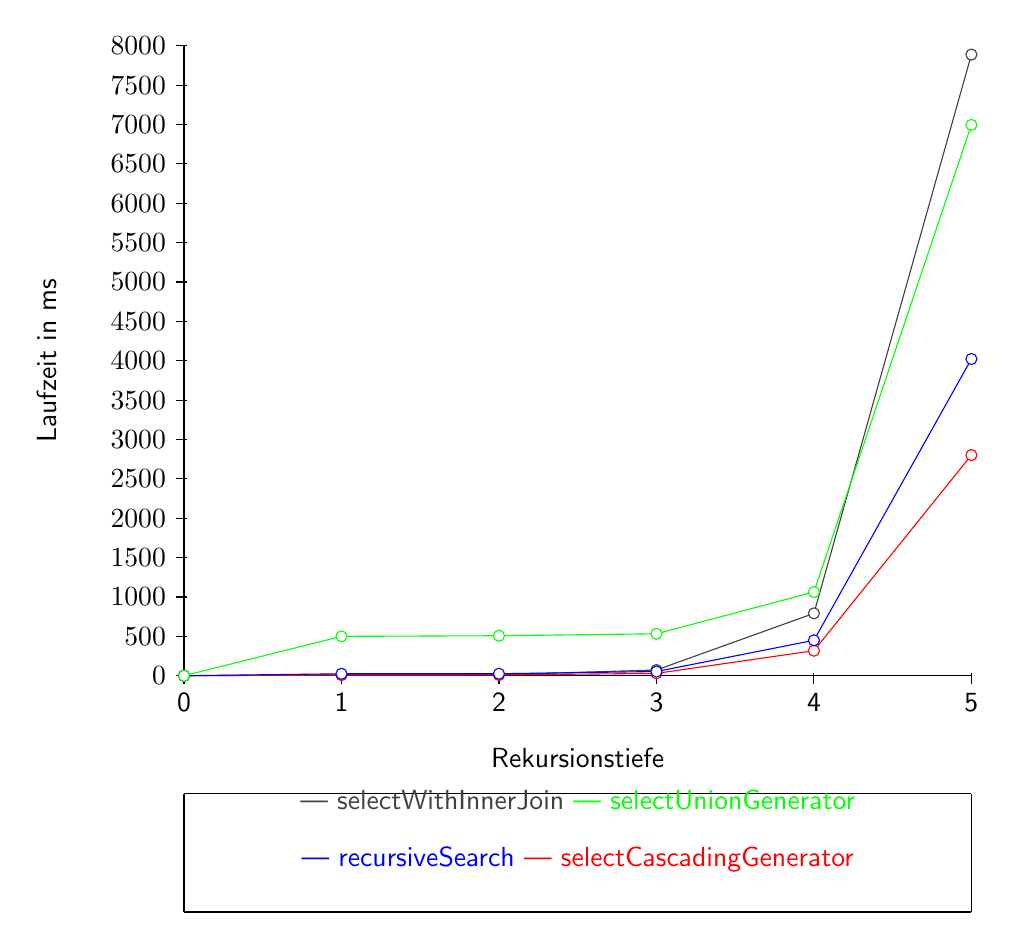
\begin{tikzpicture}[y=.5cm, x=2cm,font=\sffamily]
	%axis
	\draw (0,0) -- coordinate (x axis mid) (5,0);
	\draw (0,0) -- coordinate (y axis mid) (0,16);
	%ticks
	\foreach \x in {0,...,5}
	\draw (\x,1pt) -- (\x,-3pt)
	node[anchor=north] {\x};
	\foreach \y/\ytext in {
		0/0,
		1/500,
		2/1000,
		3/1500,
		4/2000,
		5/2500,
		6/3000,
		7/3500,
		8/4000,
		9/4500,
		10/5000,
		11/5500,
		12/6000,
		13/6500,
		14/7000,
		15/7500,
		16/8000
	}
	\draw (1pt,\y) -- (-3pt,\y) node[anchor=east] {$\ytext$};
	%labels      
	\node[below=0.8cm] at (x axis mid) {Rekursionstiefe};
	\node[rotate=90, above=1.5cm] at (y axis mid) {Laufzeit in ms};
	%plots
	%InnerJoin
	\draw[darkgray] plot[mark=*, mark options={fill=white}] 
	coordinates{(0, 0)
		(1, 11.849/500)
		(2,	13.616/500)
		(3, 72.842/500)
		(4, 792.107/500)
		(5,	7888.135/500)
	};
	%SelectGenerator
	\draw[red] plot[mark=*, mark options={fill=white}] 
	coordinates{(0, 0)
		(1, 0.018)%8.945/500
		(2,	9.875/500)
		(3, 29.855/500)
		(4, 317.921/500)%
		(5,	2802.370/500)	
	};
	%RecursiveSearch
	\draw[blue] plot[mark=*, mark options={fill=white}] 
	coordinates{(0, 0)
		(1, 24.721/500)
		(2,	25.354/500)
		(3, 53.544/500)
		(4, 449.968/500)
		(5,	4022.937/500)
	};
	%SelectWithUnion
	\draw[green] plot[mark=*, mark options={fill=white}] 
	coordinates{(0, 0)
		(1, 500.063/500)
		(2,	507.950/500)
		(3, 532.557/500)
		(4, 1062.957/500)
		(5, 6995.607/500)
	};
	
	\draw (0,-3) -- (5,-3) 
		  (0,-3) -- (0,-6)
		  (0,-6) -- (5,-6)
		  (5,-3) -- (5,-6);
	\draw[draw=none] (0,0) -- (5,0) 
	node[draw=none, midway, yshift=-4.5em]
	 {
	 	\textcolor{darkgray}{--- selectWithInnerJoin}
	 	\textcolor{green}{--- selectUnionGenerator} 
	
	};
	\draw[draw=none] (0,-3) -- (5,0) 
	node[draw=none, midway, yshift=-4.5em]
	{
		\textcolor{blue}{--- recursiveSearch} 
		\textcolor{red}{--- selectCascadingGenerator}
	};

	\end{tikzpicture}
	\caption{ relation\_livejournal\_partitioned}
\end{figure}
\begin{table}[H]
	\centering
	\begin{tabular}{l|l|l|l|l|l|}
		\cline{2-6}
		& \multicolumn{5}{|l|}{Laufzeit in MS}                                                                                                                                                  \\ \hline
		\multicolumn{1}{|l|}{\multirow{2}{2cm}{Rerkusions-tiefe}} & \multicolumn{2}{|l|}{\multirow{2}{3cm}{selectCascading Generator}} & \multirow{2}{2.8cm}{recursiveSearch} & \multirow{2}{2.5cm}{selectUnion Generator} & \multirow{2}{2.5cm}{selectInner JoinGenerator} \\
		\multicolumn{1}{|l|}{}
		& \multicolumn{2}{|l|}{}                                           &                                  &                                     &                                           \\ \hline
		
		\multicolumn{1}{|l|}{1}                                 & \multicolumn{2}{l|}{8.9415}                                      & 24.721                                                & 500.063                                                   & 11.849                                                          \\ \hline
		\multicolumn{1}{|l|}{2}                                 & \multicolumn{2}{l|}{9.875}                                       & 25.354                                                & 507.950                                                   & 13.616                                                          \\ \hline
		\multicolumn{1}{|l|}{3}                                 & \multicolumn{2}{l|}{29.855}                                      & 53.544                                                & 532.557                                                   & 72.842                                                          \\ \hline
		\multicolumn{1}{|l|}{4}                                 & \multicolumn{2}{l|}{317.921}                                     & 449.968                                               & 1062.957                                                  & 792.107                                                         \\ \hline
		\multicolumn{1}{|l|}{5}                                 & \multicolumn{2}{l|}{2802.370}                                    & 4022.937                                              & 6995.607                                                  & 7888.135                                                        \\ \hline
		
		
		
	\end{tabular}
	\caption{Laufzeit der SQLs für Tabelle relation\_livejournal\_partitioned}
\end{table}
Durch die Partitionierung ergeben sich weitere Verbesserungen in der Performance. So verringert sich die Laufzeit in der fünften Rekursionsstufe um nochmal eine Sekunde. Auffällig ist auch, dass in der partionierten Tabelle das verschachtelte Select die geringste Latenz aufweist. In den beiden anderen livejournal-Tabellen war die rekursive Stored Proceduere am schnellsten. Aufällig ist auch, dass die Partitionierung nur beim verschachtelten Select und beim InnerJoin-Select zu einer verbesserung geführt hat. Bei den beiden anderen Statements hat sich keine Verbesserung der Latenz ergeben.


\paragraph{relation\_facebook\_partitioned}\mbox{}\\
\begin{figure}[H]
	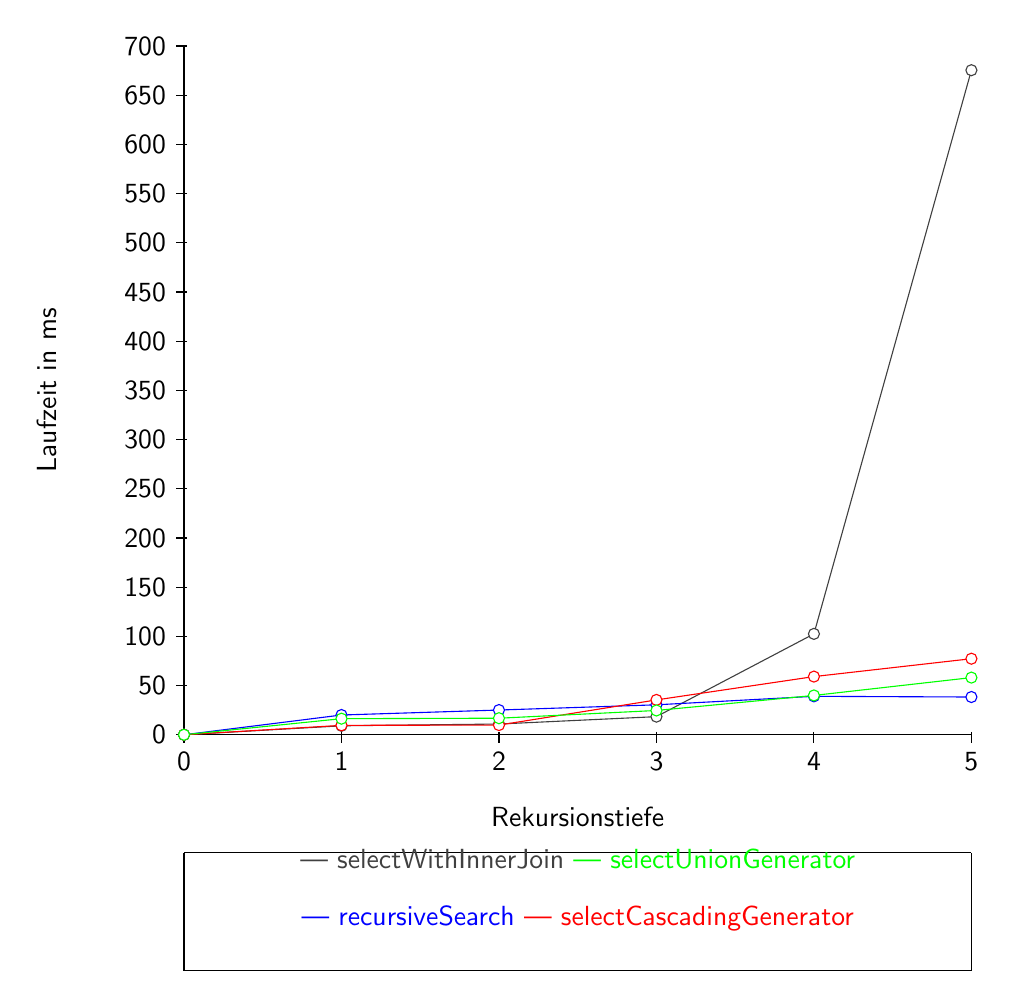
\begin{tikzpicture}[y=.0125cm, x=2cm,font=\sffamily]
	%axis
	\draw (0,0) -- coordinate (x axis mid) (5,0);
	\draw (0,0) -- coordinate (y axis mid) (0,700);
	%ticks
	\foreach \x in {0,...,5}
	\draw (\x,1pt) -- (\x,-3pt)
	node[anchor=north] {\x};
	\foreach \y in {0,50,...,700}
	\draw (1pt,\y) -- (-3pt,\y)
	node[anchor=east] {\y}; 
	%labels      
	\node[below=0.8cm] at (x axis mid) {Rekursionstiefe};
	\node[rotate=90, above=1.5cm] at (y axis mid) {Laufzeit in ms};
	%plots
	\draw[darkgray] plot[ mark=*, mark options={fill=white}] 
	coordinates{(0, 0)
		(1, 9.097)
		(2, 10.898)
		(3, 18.393)
		(4, 102.515)
		(5, 675.363)
	};
	
	\draw[blue] plot[ mark=*, mark options={fill=white}] 
	coordinates{(0, 0)
		(1, 20.057)
		(2, 25.119)
		(3, 30.430)
		(4, 39.050)
		(5, 38.354)
	};
	\draw[red] plot[ mark=*, mark options={fill=white}] 
	coordinates{(0, 0)
		(1, 9.550)
		(2, 9.838)
		(3, 35.418)
		(4, 59.112)
		(5, 77.279)
	};
	\draw[green] plot[ mark=*, mark options={fill=white}] 
	coordinates{(0, 0)
		(1, 16.339)
		(2, 16.807)
		(3, 24.669)
		(4, 39.953)
		(5, 58.086)
	};
	
	\draw (0,-120) -- (5,-120) 
	(0,-120) -- (0,-240)
	(0,-240) -- (5,-240)
	(5,-120) -- (5,-240);
	\draw[draw=none] (0,0) -- (5,0) 
	node[draw=none, midway, yshift=-4.5em]
	{
		\textcolor{darkgray}{--- selectWithInnerJoin}
		\textcolor{green}{--- selectUnionGenerator} 
		
	};
	\draw[draw=none] (0,-120) -- (5,0) 
	node[draw=none, midway, yshift=-4.5em]
	{
		\textcolor{blue}{--- recursiveSearch} 
		\textcolor{red}{--- selectCascadingGenerator}
	};
	\end{tikzpicture}
	\caption{relation\_facebook\_partitioned}
\end{figure}

\begin{table}[H]
	\centering
	\begin{tabular}{l|l|l|l|l|l|}
		\cline{2-6}
		& \multicolumn{5}{|l|}{Laufzeit in MS}                                                                                                                                                  \\ \hline
		\multicolumn{1}{|l|}{\multirow{2}{2cm}{Rerkusions-tiefe}} & \multicolumn{2}{|l|}{\multirow{2}{3cm}{selectCascading Generator}} & \multirow{2}{2.8cm}{recursiveSearch} & \multirow{2}{2.5cm}{selectUnion Generator} & \multirow{2}{2.5cm}{selectInner JoinGenerator} \\
		\multicolumn{1}{|l|}{}
		& \multicolumn{2}{|l|}{}                                           &                                  &                                     &                                           \\ \hline
		
\multicolumn{1}{|l|}{1}                                 & \multicolumn{2}{l|}{9.550}                                       & 20.057                                                & 16.339                                                    & 9.097                                                           \\ \hline
\multicolumn{1}{|l|}{2}                                 & \multicolumn{2}{l|}{9.838}                                       & 25.119                                                & 16.807                                                    & 10.898                                                          \\ \hline
\multicolumn{1}{|l|}{3}                                 & \multicolumn{2}{l|}{35.418}                                      & 30.430                                                & 24.669                                                    & 18.393                                                          \\ \hline
\multicolumn{1}{|l|}{4}                                 & \multicolumn{2}{l|}{59.112}                                      & 39.050                                                & 39.953                                                    & 102.515                                                         \\ \hline
\multicolumn{1}{|l|}{5}                                 & \multicolumn{2}{l|}{77.279}                                      & 38.354                                                & 58.086                                                    & 675.363                                                         \\ \hline

		
		
	\end{tabular}
	\caption{Laufzeit der SQLs für Tabelle relation\_facebook\_partitioned}
\end{table}

Durch die Partitionierung der Tabellen ergibt sich keine weitere Verbesserung gegenüber der Tabelle mit den Indices. Der InnerJoin weißt mit einer Latenz von 675 Millisekunden sogar einen deutlich schlechteren Wert auf.


\paragraph{relation\_wiki\_vote\_partitioned}\mbox{}\\
\begin{figure}[H]
	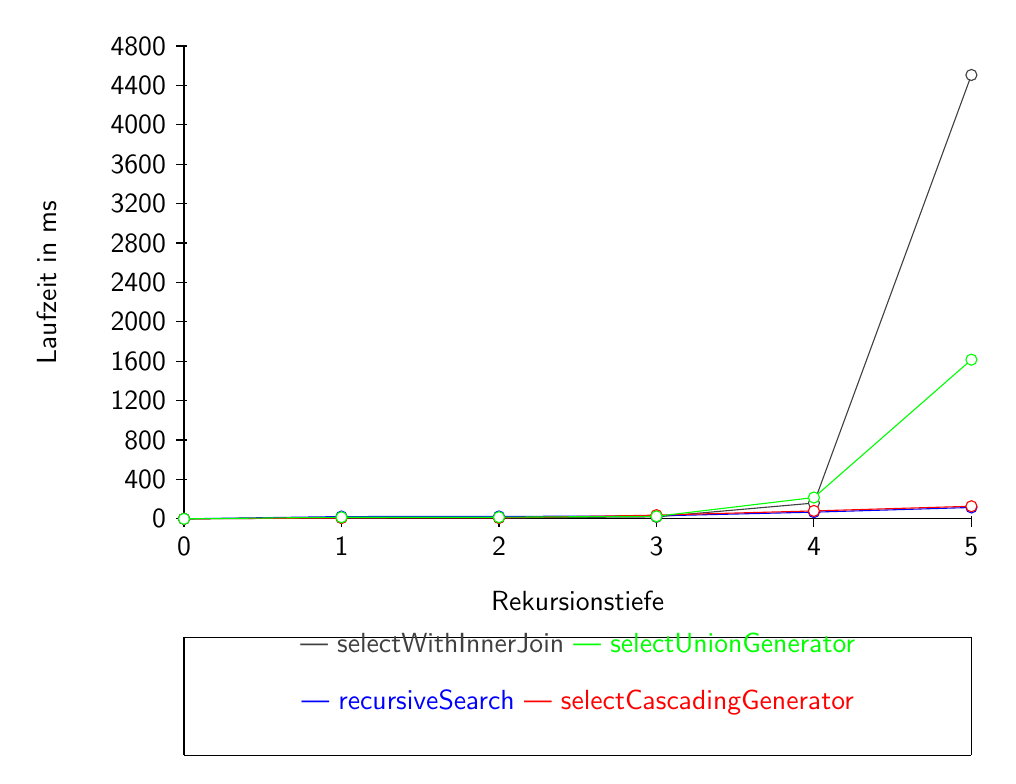
\begin{tikzpicture}[y=.00125cm, x=2cm,font=\sffamily]
	%axis
	\draw (0,0) -- coordinate (x axis mid) (5,0);
	\draw (0,0) -- coordinate (y axis mid) (0,4800);
	%ticks
	\foreach \x in {0,...,5}
	\draw (\x,1pt) -- (\x,-3pt)
	node[anchor=north] {\x};
	\foreach \y in {0,400,...,4800}
	\draw (1pt,\y) -- (-3pt,\y)
	node[anchor=east] {\y}; 
	%labels      
	\node[below=0.8cm] at (x axis mid) {Rekursionstiefe};
	\node[rotate=90, above=1.5cm] at (y axis mid) {Laufzeit in ms};
	%plots
	\draw[darkgray] plot[ mark=*, mark options={fill=white}] 
	coordinates{(0, 0)
		(1, 8.882)
		(2, 9.694)
		(3, 20.019)
		(4, 160.368)
		(5, 4505.545)
	};
	
	\draw[blue] plot[ mark=*, mark options={fill=white}] 
	coordinates{(0, 0)
		(1, 23.059)
		(2, 24.221)
		(3, 29.832)
		(4, 67.963)
		(5, 115.465)
	};
	\draw[red] plot[ mark=*, mark options={fill=white}] 
	coordinates{(0, 0)
		(1, 9.169)
		(2, 9.538)
		(3, 37.563)
		(4, 80.343)
		(5, 127.839)
	};
	\draw[green] plot[ mark=*, mark options={fill=white}] 
	coordinates{(0, 0)
		(1, 16.152)
		(2, 16.649)
		(3, 25.806)
		(4, 216.439)
		(5,1615.686)
	};
	
	\draw (0,-1200) -- (5,-1200) 
	(0,-1200) -- (0,-2400)
	(0,-2400) -- (5,-2400)
	(5,-1200) -- (5,-2400);
	\draw[draw=none] (0,0) -- (5,0) 
	node[draw=none, midway, yshift=-4.5em]
	{
		\textcolor{darkgray}{--- selectWithInnerJoin}
		\textcolor{green}{--- selectUnionGenerator} 
		
	};
	\draw[draw=none] (0,-1200) -- (5,0) 
	node[draw=none, midway, yshift=-4.5em]
	{
		\textcolor{blue}{--- recursiveSearch} 
		\textcolor{red}{--- selectCascadingGenerator}
	};
	\end{tikzpicture}
	\caption{relation\_wiki\_vote\_partitioned}
\end{figure}

\begin{table}[H]
	\centering
	\begin{tabular}{l|l|l|l|l|l|}
		\cline{2-6}
		& \multicolumn{5}{|l|}{Laufzeit in MS}                                                                                                                                                  \\ \hline
		\multicolumn{1}{|l|}{\multirow{2}{2cm}{Rerkusions-tiefe}} & \multicolumn{2}{|l|}{\multirow{2}{3cm}{selectCascading Generator}} & \multirow{2}{2.8cm}{recursiveSearch} & \multirow{2}{2.5cm}{selectUnion Generator} & \multirow{2}{2.5cm}{selectInner JoinGenerator} \\
		\multicolumn{1}{|l|}{}
		& \multicolumn{2}{|l|}{}                                           &                                  &                                     &                                           \\ \hline
		
\multicolumn{1}{|l|}{1}                                 & \multicolumn{2}{l|}{9.169}                                       & 23.059                                                & 16.152                                                    & 8.882                                                           \\ \hline
\multicolumn{1}{|l|}{2}                                 & \multicolumn{2}{l|}{9.538}                                       & 24.221                                                & 16.649                                                    & 9.694                                                           \\ \hline
\multicolumn{1}{|l|}{3}                                 & \multicolumn{2}{l|}{37.563}                                      & 29.832                                                & 25.806                                                    & 20.019                                                          \\ \hline
\multicolumn{1}{|l|}{4}                                 & \multicolumn{2}{l|}{80.343}                                      & 67.963                                                & 216.439                                                   & 160.368                                                         \\ \hline
\multicolumn{1}{|l|}{5}                                 & \multicolumn{2}{l|}{127.839}                                     & 115.465                                               & 1615.686                                                  & 4505.545                                                        \\ \hline

		
		
	\end{tabular}
	\caption{Laufzeit der SQLs für Tabelle relation\_wiki\_vote\_partitioned}
\end{table}

Durch die Partitionierung der relation\_wiki\_vote Tabelle verschlechtern sich in der fünften Rekursionsstufe alle Statements bis auf die Rekursive Suche. Insgesamt ergibt sich aber keine Verbesserung, da die Rekursive Suche auf der partionierten Tabelle gleich schnell ist wie das verschachtelte Select auf der nicht partionierten Tabelle mit den Indices.

\newpage

\paragraph{relation\_youtube\_partitioned}\mbox{}\\

\begin{figure}[H]
	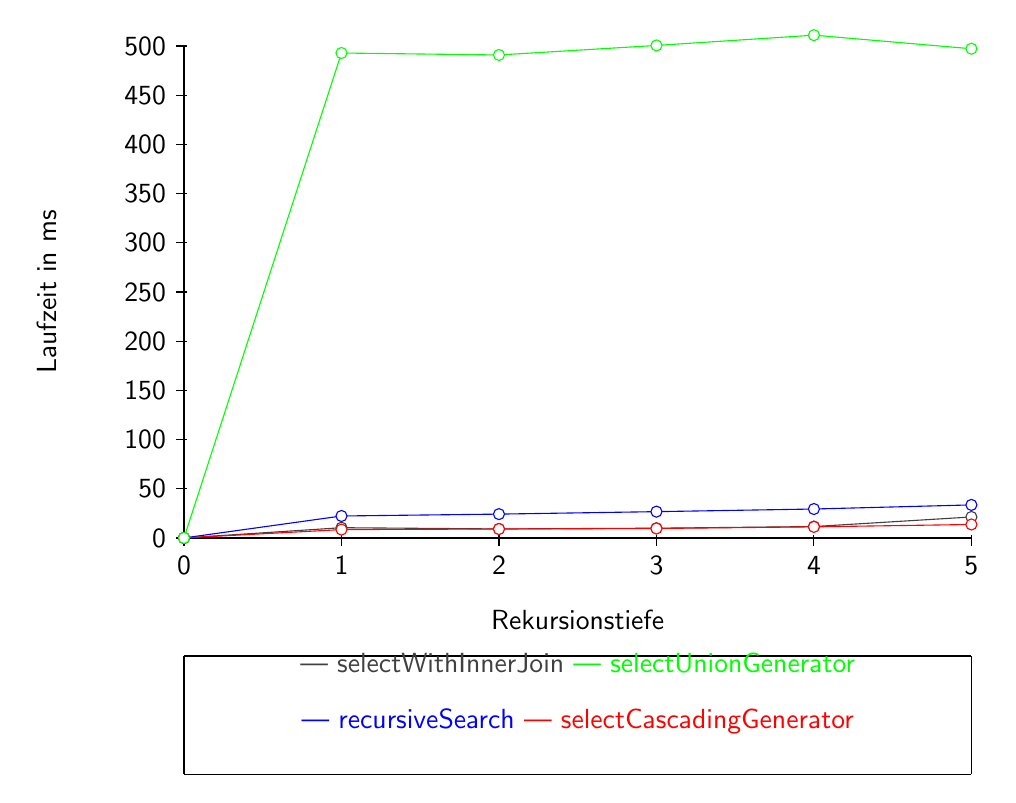
\begin{tikzpicture}[y=.0125cm, x=2cm,font=\sffamily]
	%axis
	\draw (0,0) -- coordinate (x axis mid) (5,0);
	\draw (0,0) -- coordinate (y axis mid) (0,500);
	%ticks
	\foreach \x in {0,...,5}
	\draw (\x,1pt) -- (\x,-3pt)
	node[anchor=north] {\x};
	\foreach \y in {0,50,...,500}
	\draw (1pt,\y) -- (-3pt,\y)
	node[anchor=east] {\y}; 
	%labels      
	\node[below=0.8cm] at (x axis mid) {Rekursionstiefe};
	\node[rotate=90, above=1.5cm] at (y axis mid) {Laufzeit in ms};
	%plots
	\draw[darkgray] plot[ mark=*, mark options={fill=white}] 
	coordinates{(0, 0)
		(1, 10.423)
		(2, 9.162)
		(3, 9.909)
		(4, 11.589)
		(5, 21.320)
	};
	
	\draw[blue] plot[ mark=*, mark options={fill=white}] 
	coordinates{(0, 0)
		(1, 22.322)
		(2, 24.235)
		(3, 26.731)
		(4, 29.409)
		(5, 33.586)
	};
	\draw[red] plot[ mark=*, mark options={fill=white}] 
	coordinates{(0, 0)
		(1, 8.505)
		(2, 9.090)
		(3, 9.629)
		(4, 11.286)
		(5, 13.694)
	};
	\draw[green] plot[ mark=*, mark options={fill=white}] 
	coordinates{(0, 0)
		(1, 492.834)
		(2, 490.843)
		(3, 500.531)
		(4, 510.964)
		(5, 497.172)
	};
	
	\draw (0,-120) -- (5,-120) 
	(0,-120) -- (0,-240)
	(0,-240) -- (5,-240)
	(5,-120) -- (5,-240);
	\draw[draw=none] (0,0) -- (5,0) 
	node[draw=none, midway, yshift=-4.5em]
	{
		\textcolor{darkgray}{--- selectWithInnerJoin}
		\textcolor{green}{--- selectUnionGenerator} 
		
	};
	\draw[draw=none] (0,-120) -- (5,0) 
	node[draw=none, midway, yshift=-4.5em]
	{
		\textcolor{blue}{--- recursiveSearch} 
		\textcolor{red}{--- selectCascadingGenerator}
	};
	\end{tikzpicture}
	\caption{ relation\_youtube\_partitioned}
\end{figure}

\begin{table}[H]
	\centering
	\begin{tabular}{l|l|l|l|l|l|}
		\cline{2-6}
		& \multicolumn{5}{|l|}{Laufzeit in MS}                                                                                                                                                  \\ \hline
		\multicolumn{1}{|l|}{\multirow{2}{2cm}{Rerkusions-tiefe}} & \multicolumn{2}{|l|}{\multirow{2}{3cm}{selectCascading Generator}} & \multirow{2}{2.8cm}{recursiveSearch} & \multirow{2}{2.5cm}{selectUnion Generator} & \multirow{2}{2.5cm}{selectInner JoinGenerator} \\
		\multicolumn{1}{|l|}{}
		& \multicolumn{2}{|l|}{}                                           &                                  &                                     &                                           \\ \hline
		
		\multicolumn{1}{|l|}{1}                                 & \multicolumn{2}{l|}{8.505}                                       & 22.322                                                & 492.834                                                   & 10.423                                                          \\ \hline
		\multicolumn{1}{|l|}{2}                                 & \multicolumn{2}{l|}{9.090}                                       & 24.235                                                & 490.843                                                   & 9.162                                                           \\ \hline
		\multicolumn{1}{|l|}{3}                                 & \multicolumn{2}{l|}{9.629}                                       & 26.731                                                & 500.531                                                   & 9.909                                                           \\ \hline
		\multicolumn{1}{|l|}{4}                                 & \multicolumn{2}{l|}{11.286}                                      & 29.409                                                & 510.964                                                   & 11.589                                                          \\ \hline
		\multicolumn{1}{|l|}{5}                                 & \multicolumn{2}{l|}{13.694}                                      & 33.586                                                & 497.172                                                   & 21.320                                                          \\ \hline
		
	\end{tabular}
	\caption{Laufzeit der SQLs für Tabelle relation\_youtube\_partitioned}
\end{table}

Durch die Partitionierung ergeben sich weitere Verbesserungen in der Laufzeit. Das verschachtelte Select sowie der InnerJoin verbessern sich deutlich. Lediglich das Standard-SQL verschlechtert sich deutlich. Jeoch bleibt die Latenz über alle Rekursionss mit ungefähr 500 Millisekunden Stufen ungefähr konstant.  Mit 13.6 Millisekdunden ist das verschachtelte Select in der fünften Rekursionstufe am schnellsten.   

%\subsection{Standard SQL}

%\subsection{Stored Procedures}
%\subsection{PL/SQL-Recursion}
%\subsection{Datenbankzugriffe}
%\subsection{Zugriffsart Aggregation}
%\subsection{Zugriffsart Traversierung}
\subsection{Interpretation der Ergebnisse}

Es ist auffallend das die Laufzeit der Statements sehr stark an der Anzahl der Eingabeknoten abhängig ist und die größe der Tabellen eher nachrangig ist. So ist die relations\_youtube Tabelle deutlich größer als die relation\_epinions Tabelle, jedoch ist die Latenz der Statements in der fünften Rekursion für die relations\_youtube Tabelle deutlich geringer als für die der relation\_epinions Tabelle.  

Bei der relation\_epinions Tabelle werden in der vierten Iteration 29184 Zeilen zurückgegeben, die dann in der fünften Iteration als Input benutzt werden. Bei der relations\_youtube Tabelle sind es nur 760. Entsprechend sind die Unterschiede in der Latenz in der fünften Rekursionsstufe. Für die Youtube-Daten werden im besten Fall nur 14 Millisekunden benötigt, bei den Epinions-Daten sind es 505 Millisekunden.

Weiterhin zeigt sich, dass das InnerJoin-Statement in fast allen Fällen in der fünften Rekursionsstufe die schlechteste Wahl darstellt. Besonders bei den Wikipedia und Epinions-Daten wird dies sehr deutlich.
